\documentclass[10pt,conference,compsocconf]{IEEEtran}

\usepackage{hyperref}
\usepackage{graphicx}
\usepackage{xcolor}
\usepackage{blindtext, amsmath, comment, epsfig }
\usepackage{caption}
\usepackage{subcaption} % or subfig
\usepackage{cleveref} % cref
\usepackage{amsfonts} 
\usepackage{algorithmic}
\usepackage{cite}
\usepackage[utf8]{inputenc}


\IEEEaftertitletext{\vspace{-1\baselineskip}}

\usepackage{scalerel}
\DeclareMathOperator*{\concat}{\scalerel*{||}{\sum}}

%\DeclareMathOperator*{\barr}{\scalerel*{\maltese}{\textstyle\sum}}

\title{\Large GeoPKI \vspace{-1.1em}}
% \author{}
\date{}



\ifdefined\final
\newcommand{\todo}[1]{}
\newcommand{\ck}[1]{}
\newcommand{\ckrm}[1]{}
\newcommand{\chrissy}[1]{}
\else
\newcommand{\todo}[1]{\textcolor{red}{\emph{\textbf{[TODO: }#1\textbf{]}}}}
\newcommand{\ck}[1]{\textcolor{violet}{\emph{\textbf{cyrill: }#1}}}
\newcommand{\ckrm}[1]{\textcolor{violet}{\emph{\textbf{cyrill remove:} ``#1''}}}
\newcommand{\chrissy}[1]{\textcolor{blue}{\emph{\textbf{chrissy: }#1}}}
\newcommand{\nico}[1]{\textcolor{orange}{\emph{\textbf{nico: }#1}}}
\fi

\begin{document}

\makeatletter
\@twocolumnfalse
\maketitle
\@twocolumntrue
\makeatother

%\begin{abstract}
%\end{abstract}


% \section{Introduction}
% \label{introduction}

\section{Model}
\label{sec:model}

The earth ellipsoid model of the existing world geodetic system 84 (WGS84) \cite{noauthor_nga_nodate} is used.
WGS84 defines the \emph{semi-major axis} (half of the largest diameter of an ellipsoid, at the equator) $a$ to be $6'378'137.0$~meters \cite{noauthor_nga_nodate}. The \emph{semi-minor axis} (the polar radius) $b$ is defined as $6'356'752.3142~$meters \cite{noauthor_nga_nodate}.
Standard polar coordinates (longitude, latitude) are used for referencing points on the planet's two-dimensional surface and a third coordinate, altitude, extends this to three dimensions.
Longitude, latitude and altitude together refer to a unique point in three-dimensions.

Each of the three coordinates is discretized in a way that preserves meter-precision in the worst case.
With the semi-major axis $a$, the maximum circumference of the ellipsoid equals $=2 a \pi$~meters.
Using base two, $B_{x}:= \left\lceil \log_2(2 a \pi) \right\rceil = 26$ bits for the longitude thus suffice to represent each possible meter value in the worst case.
Let $C_{x} := 2^{B_{x}} - 1$ denote the maximum discretized value for the longitude.
For the latitude the circumference is $2 b \pi$~meters but we only need to be able to represent half of it, so $b \pi$.
Thus $\left\lceil\log_2(C_y)\right\rceil = 25 =: B_{y}$ bits suffice.
Analogously to $C_{x}$, let $C_y := 2^{B_{y}} - 1$ the maximum discretized value for the latitude.
For altitude there is no natural bound so one has to be fixed.
At the time of writing, the highest point on earth is below $10'000$~meters above sea level \cite{us_department_of_commerce_what_nodate} and the lowest layer of earth's atmosphere, the troposphere, extends to about $18$~km \cite{dhaka_chapter_2023}.
The Mariana Trench at about $10'000$~m below sea level \cite{gardner_so_2014} is likely a bound not exceeded in the near future.
The necessity of allowing volumes below sea level arises from countries such as the Netherlands where parts of the surface's altitude is below sea level \cite{kabat_climate_2005} .
Moreover in the future, below sea level research stations might be built.
Thus the range starting at a depth of $D:=-10'000$~m up to an altitude of $20'000$~m above sea level should cover any current and near-future needs.
Covering this range requires $B_{z} := \left\lceil \log_2(H - D) \right\rceil = 15$ bits.
In fact using $B_z$ bits starting at $D$ will cover the range from $D$ to $D + (2^{B_{z}} - 1) = 22'767 := H$.
Complications might arise from distance calculations when using sea level as a reference as the sea level is not the same in all places and will increase in the future.
Thus instead of using sea level as a reference, the geodetic altitude defined by WGS84~\cite{noauthor_nga_nodate} is used.
Given the geoid's surface in WGS84 is about at the mean sea level (MSL), the range $[D, H]$ can be left as is.
While it does not exactly cover the range described range with respect to local sea level, it approximates it.

\section{Data Structure}
\label{sec:data-structure}

Inspired by F-PKI~\cite{chuat_f-pki_2022}, a sparse merkle hash tree (SMT) is used.
Each leaf represents a full discretized coordinate using $B := \cdot B_{x} + B_{y} + B_{z} = 66$ bits resulting in a total of $2^{B}$ leaves.
To have spatially close points somewhat close together in the SMT, the space-filling $Z$-order curve is used to sort the three dimensional locations in one dimension \cite{morton_computer_1966}.
An example with $B_{x} = B{y} = B_{z} = 2$ is shown in \Cref{fig:z-curve-example:two-bits}.
GeoPKI uses a slightly modified 3D Z-order curve:
Rather than using the full 3D Z-order curve, a 2D Z-order curve over the longitude and latitude is used and points with the same longitude and latitude but different altitude are put in sequence.
While this leads to spatially close points being further apart in the 1-dimensional sorting, this modification allows for shorter proofs under some assumptions (will be discussed in \Cref{sec:optimizations}) and even results in a nicer binary representation.
\Cref{fig:z-curve-example:two-bits-optim} contrasts this modification with the standard 3D Z-order curve shown in \Cref{fig:z-curve-example:two-bits}.

\subsection{Leaf Binary Format}
\label{sec:data-structure:leaf-binary}
Each leaf of the SMT corresponds to a point and the tree leaves are sorted lexicographically by their binary representation in ascending order.
A point tuple $p := (x,y,z)$ at longitude $x$, latitude $y$ and altitude $z$ with
\begin{align*}
	(x, y, z) &\in [-180, 180] \times [-90, 90] \times [D, H]
\end{align*}

is first discretized to integer coordinates as follows:

\begin{align}
\begin{split}
\label{eq:discretization}
p' :&=
(x_d,y_d, z_d)
\\
& =
\left(
%
\left\lfloor
\frac{x + 180}{360} \cdot C_x
\right\rfloor,
%
\left\lfloor
\frac{y + 90}{180} \cdot C_y
\right\rfloor,
%
\left\lfloor
z - D
\right\rfloor
%
\right)
\end{split}
\end{align}

After this transformation the following folds:

\begin{align*}
	p' &\in [0, 2^{B_x}) \times [0, 2^{B_y}) \times [0, 2^{B_z})
\end{align*}

This formula holds since the first term in the longitude and latitude tuples can be at most $1$ and since $C_x$ and $C_y$ are the maximum values that can be represented using $B_x$ and $B_y$ bits, respectively.
Moreover $H - D = 2^{B_z} - 1$ holds meaning the altitude can be represented using $B_z$ bits.
The three resulting integer numbers can now be represented using $B_{x}$, $B_{y}$ and $B_z$ bits, respectively. Let $p'' := (x_b, y_b, z_b)$ be their big-endian integer binary encoding with
\begin{align*}
	p'' &\in \{0,1\}^{B_{x}} \times \{0,1\}^{B_{y}} \times \{0,1\}^{B_z}
\end{align*}

For $c \in \{x, y, z\}$ and for any integer $i \in \{0, ..., B_c-1\}$, let $c_{b,i}$ denote the $i$-th bit of $c_{b}$. Moreover let $||$ denote the concatenation operator.
The binary representation $p_b$ of the point $p$ is then defined as
\begin{align*}
	p_b = \left(\concat_{i=0}^{B_{y} - 1} x_{b,i} || y_{b,i} \right) || x_{b,B_{x}-1} || \left(\concat_{i=0}^{B_{z}-1} z_{b,i} \right)
\end{align*}

In words, the binary representation of $p$ is the interleaving of the binary representation for the longitude and latitude concatenated to the binary representation of the altitude.

\Cref{fig:leaf-representation:binary} shows an example of this binary encoding.

% ($47.37643$, $8.54828$, $0$)

%Storing a dense SMT with $2^{B} \leq (2^{10})^7 \approx (10^3)^7 = 10^{21}$ leaves is certainly infeasible but under the assumption that most leaves are empty it seems reasonable.

\begin{figure}
    \centering
    \begin{subfigure}[t]{0.24\textwidth}
        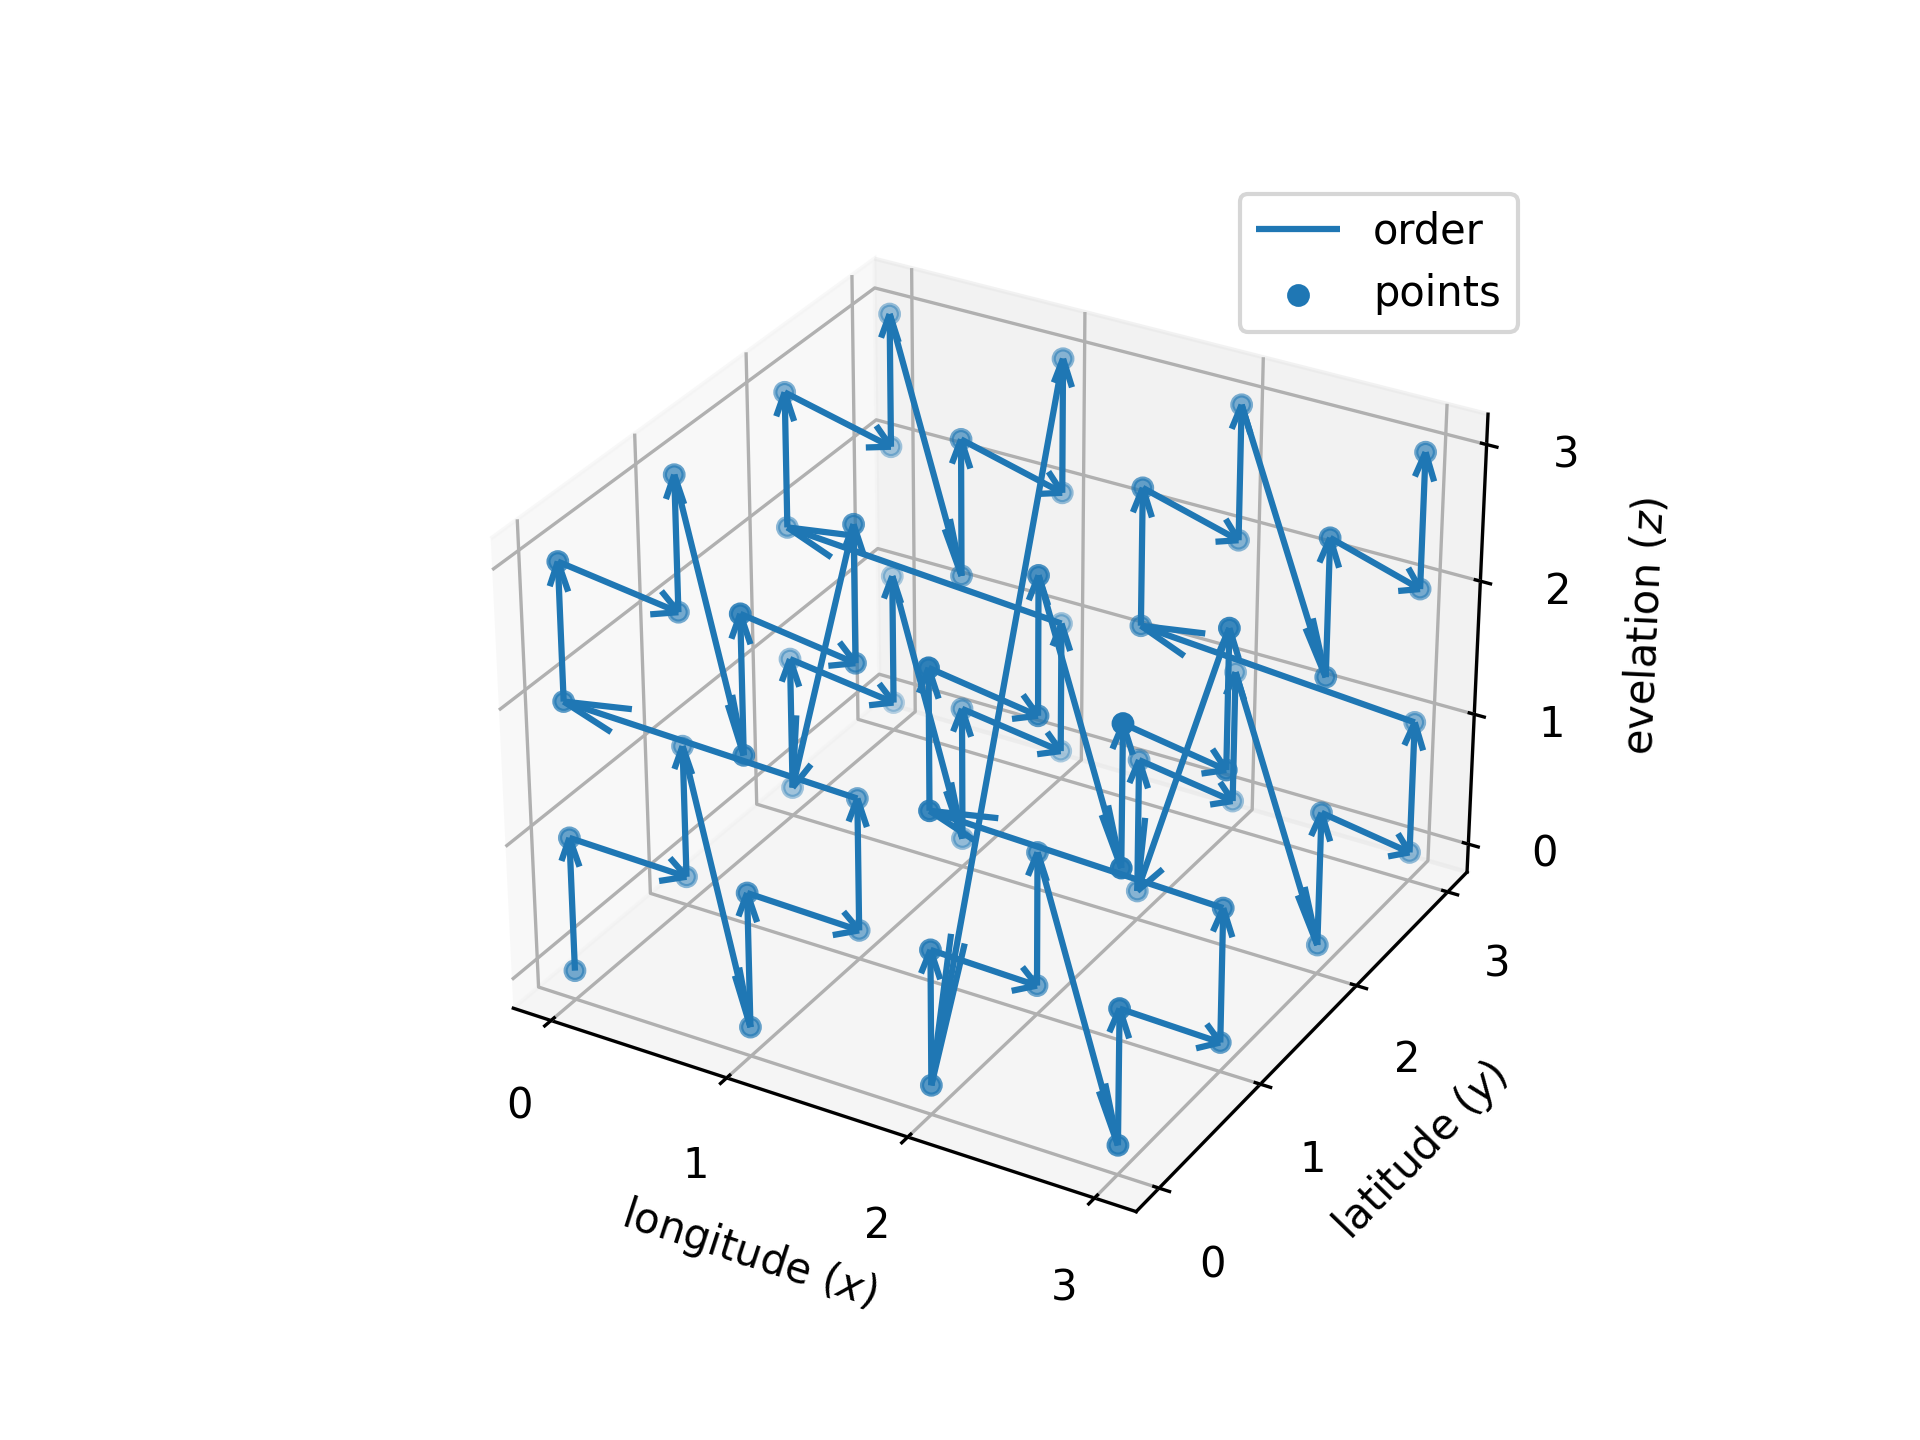
\includegraphics[width=\textwidth]{./resources/z-example/two-bits-z.png}
        \caption{3D Z-Order Curve}
        \label{fig:z-curve-example:two-bits}
    \end{subfigure}
    \hfill
    \begin{subfigure}[t]{0.24\textwidth}
        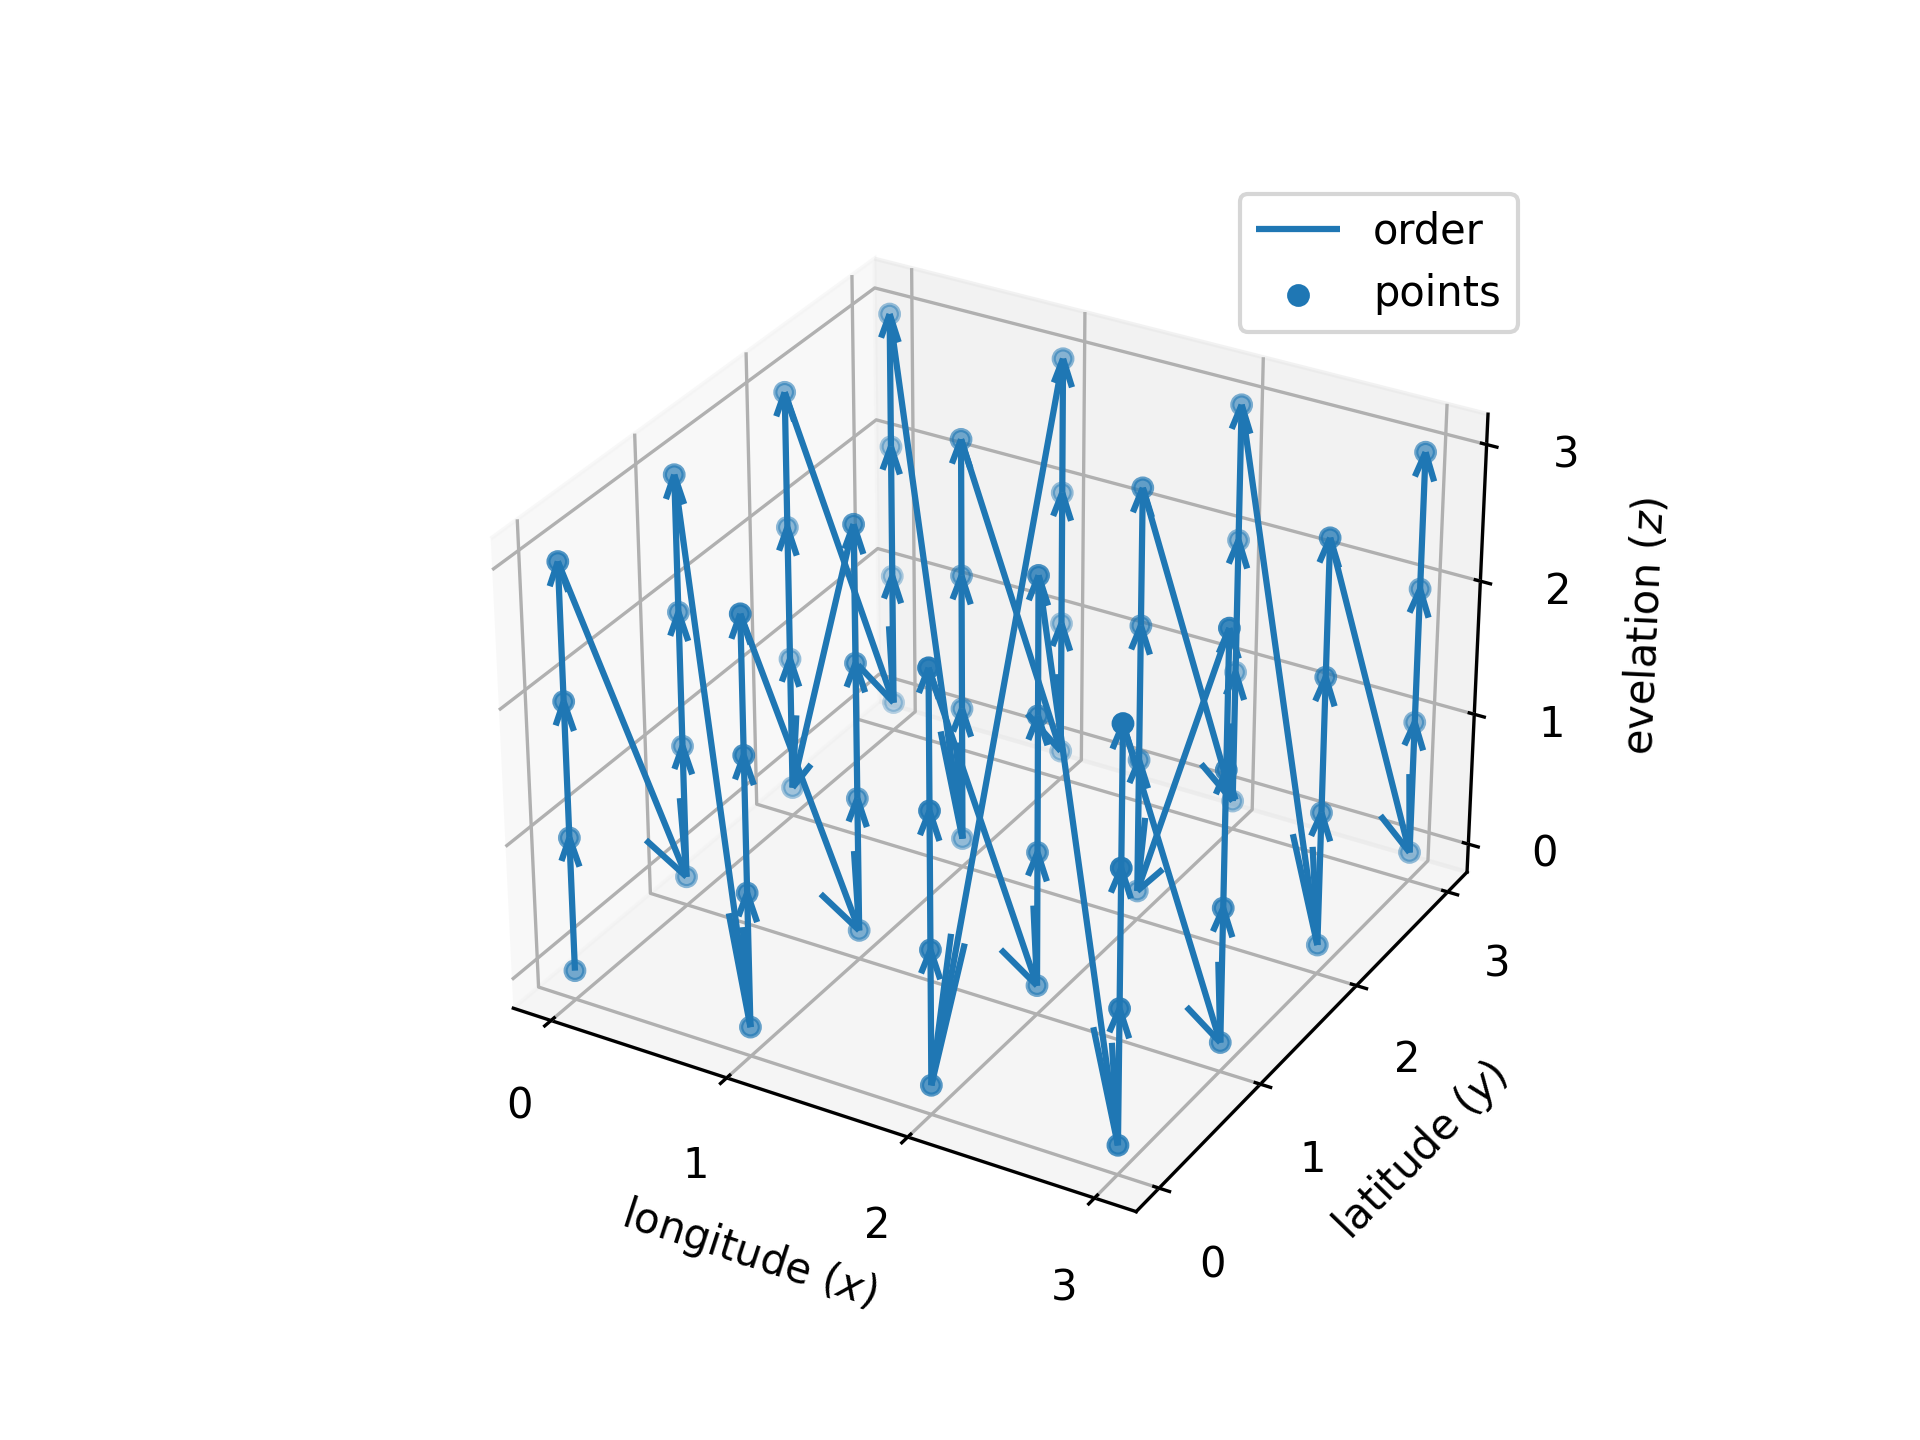
\includegraphics[width=\textwidth]{./resources/z-example/two-bits.png}
        \caption{2D Z-Order Curve with altitude in sequence}
        \label{fig:z-curve-example:two-bits-optim}
    \end{subfigure}
    \caption{
    	Difference between a standard 3D Z-order curve and the one used by GeoPKI when using two bits for all coordinates.
    }
    \label{fig:z-curve-example}
\end{figure}

\subsection{Leaf Geometric Representation}
\label{sec:data-structure:leaf-geometry}
Due to the floor functions in \Cref{eq:discretization}, the point $p''$ represents the volume where $p''$ is in the corner with the smallest coordinates in all three dimensions.
By replacing the floor functions by mathematically rounding or the ceil function the volumetric representation changes.
In case of the floor functions shown in \Cref{eq:discretization}, the point corresponding to $p''$ is
\begin{align}
\begin{split}
\label{eq:leaf-geometric-point}
\left(x_d \cdot \frac{360}{C_x} - 180,x_d \cdot \frac{180}{C_y} - 90, z_d + D\right)
\end{split}
\end{align}
and the volume represented by point $p''$ is given by
\begin{align}
\begin{split}
\label{eq:leaf-geometric-volume}
\left[x_d \cdot \frac{360}{C_x} - 180, (x_d + 1) \cdot \frac{360}{C_x} - 180\right) &\times\\
\left[y_d \cdot \frac{180}{C_y} - 90, (y_d + 1) \cdot \frac{180}{C_y} - 90\right) &\times\\
\left[z_d + D, z_d + D + 1 \right)&
\end{split}
\end{align}

\Cref{fig:leaf-representation:geometric} shows the points and the corresponding volumes in the same color.

\begin{figure}
    \centering
    \begin{subfigure}[t]{0.24\textwidth}
        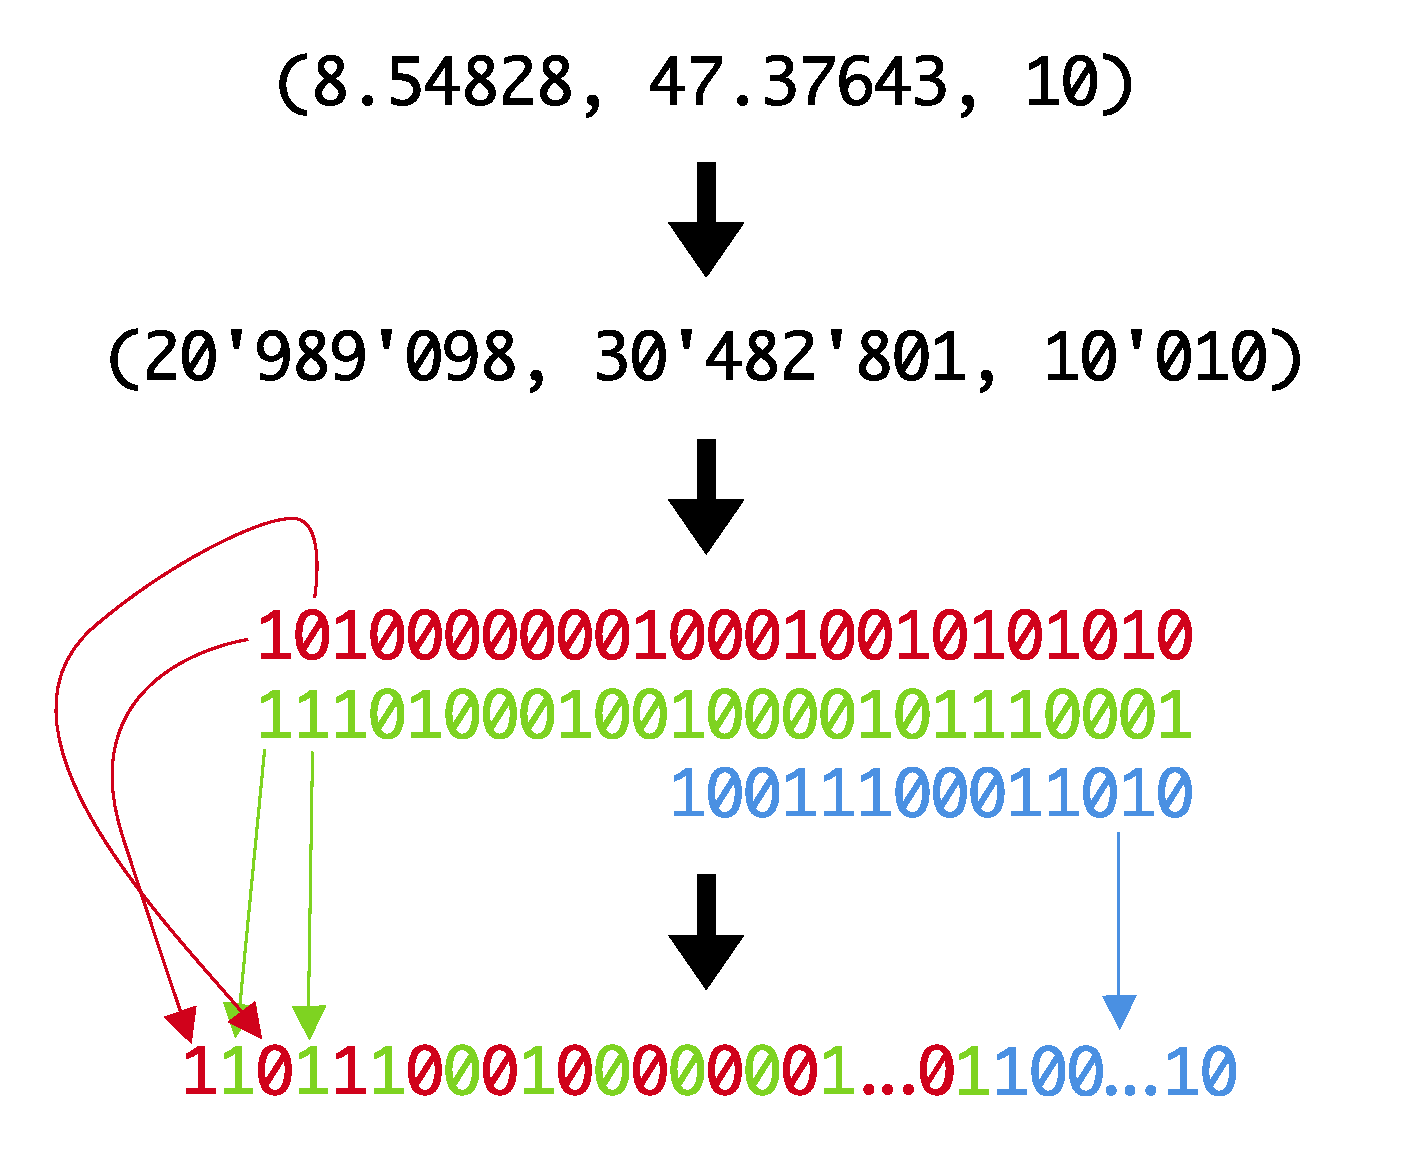
\includegraphics[width=\textwidth]{./resources/leaf-representation/binary-representation.pdf}
        \caption{Binary Representation of a (longitude, latitude, altitude) tuple.}
        \label{fig:leaf-representation:binary}
    \end{subfigure}
    \hfill
    \begin{subfigure}[t]{0.24\textwidth}
        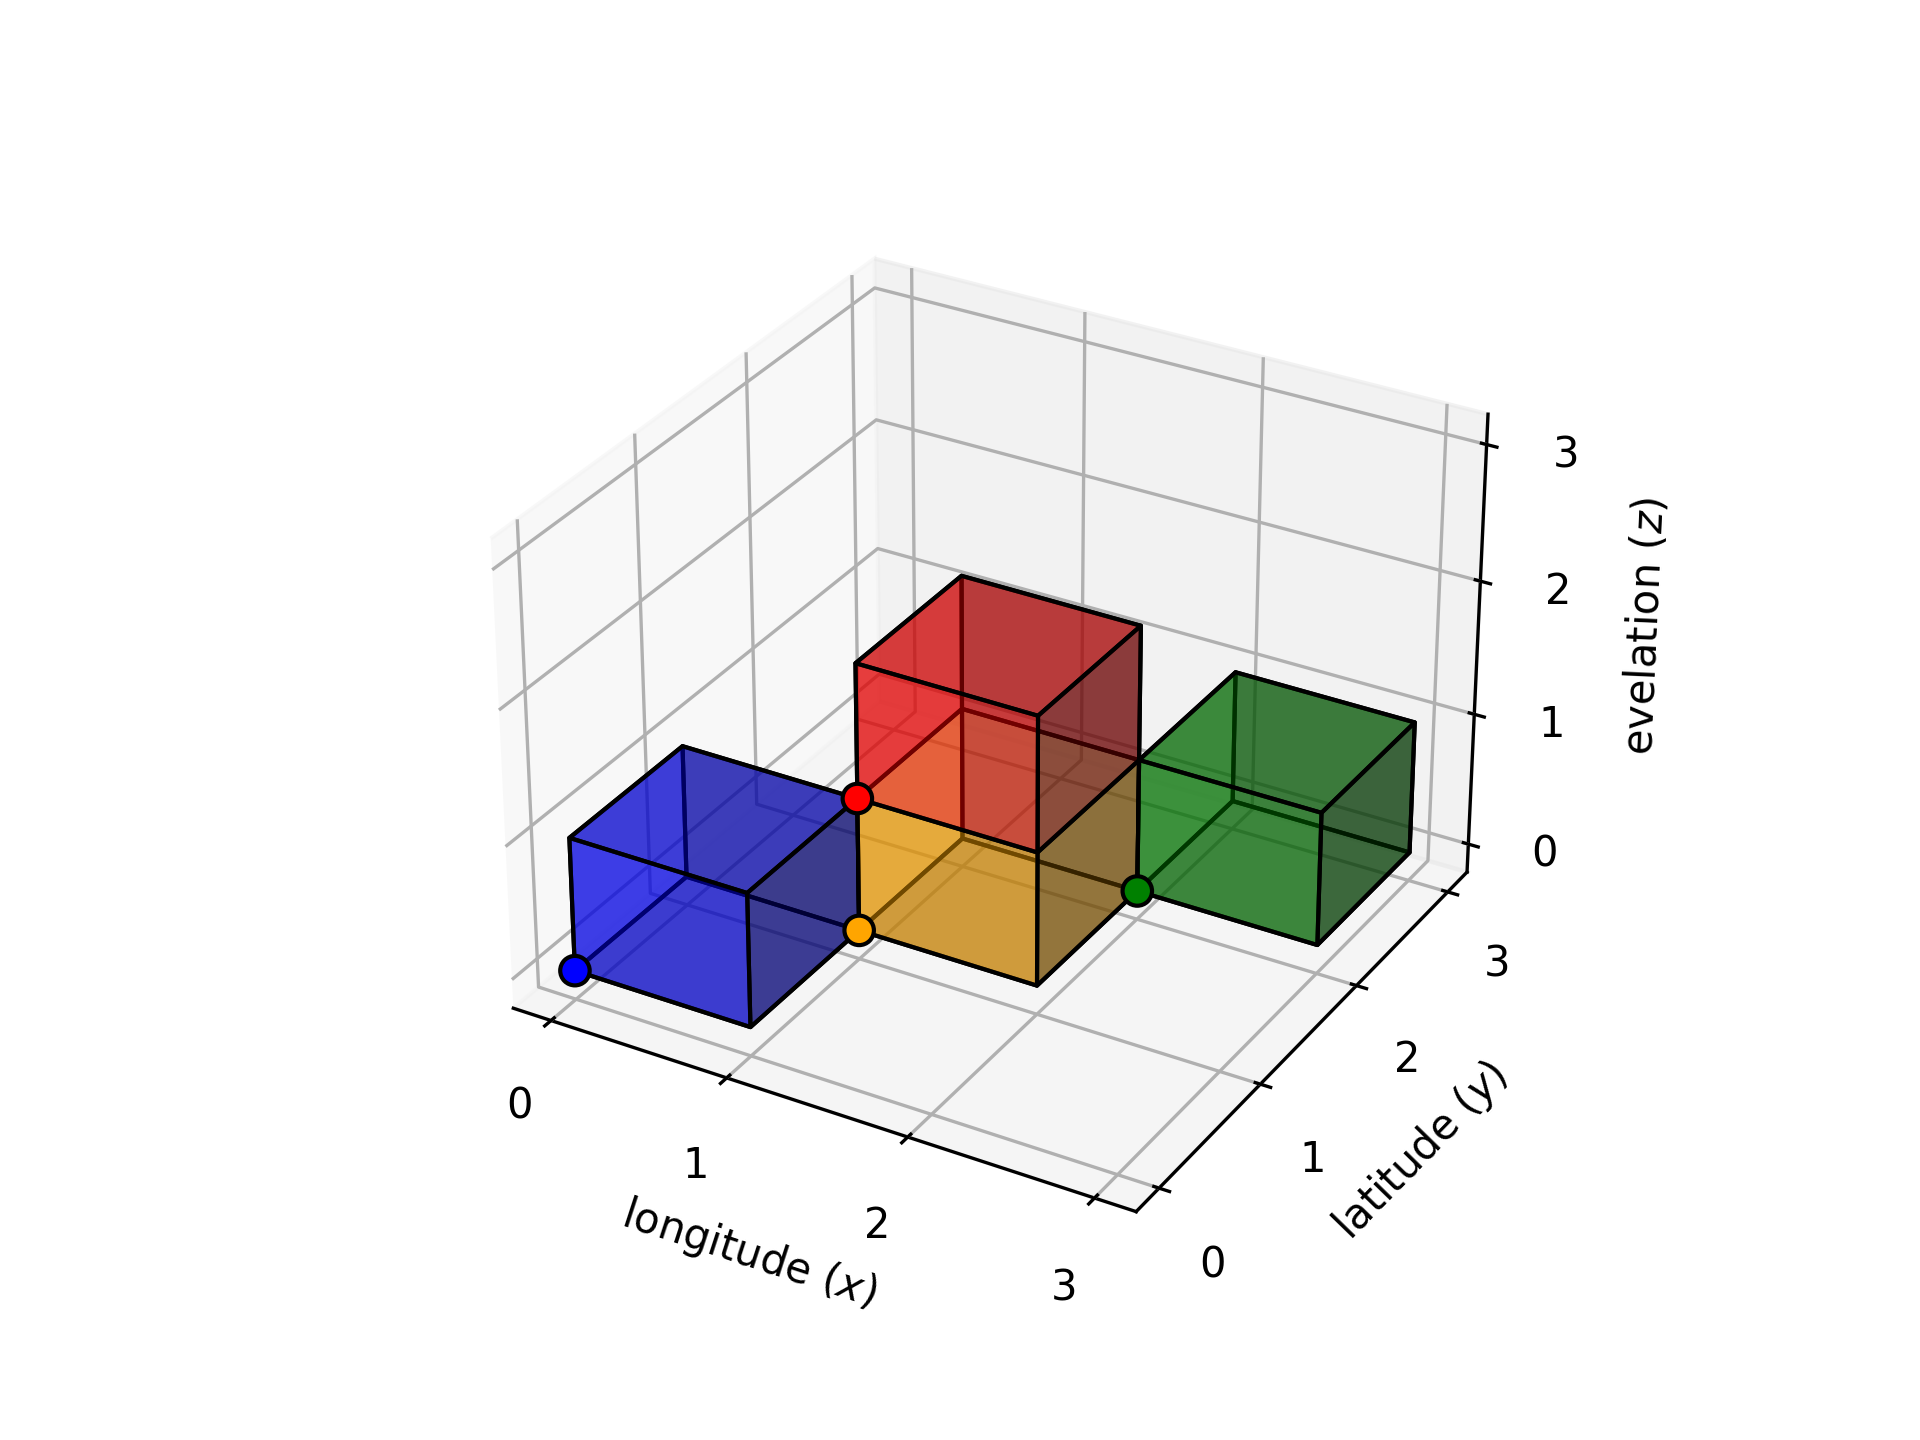
\includegraphics[width=\textwidth]{./resources/leaf-representation/geometric-representation.png}
        \caption{Geometric Representation}
        \label{fig:leaf-representation:geometric}
    \end{subfigure}
    \caption{
    	The binary and geometric representation of a leaf
    }
    \label{fig:leaf-representation}
\end{figure}

\subsection{Intermediate Nodes}
\label{sec:data-structure:intermediate}
Intermediate nodes in the SMT also correspond to a point and a volume following the same pattern as for the leaf nodes.
The bit string corresponding to an intermediate node is simply the longest common prefix of it's two children and covers the whole volume of its two children.
The left child is the node with the binary representation equal to the intermediate node one's concatenated with a zero and the right child concatenated with a one.
The formula for computing the volume becomes more complex for intermediate nodes as it requires a case distinction:
Let $s$ be the bit string of an intermediate node.

Let $l$ be the length of $s$.
Let $s_x$, $s_y$, $s_z$ be the bit prefixes encoded in $s$ corresponding to the longitude, latitude and altitude, respectively.
Moreover let $l_x$, $l_y$ and $l_z$ be the lengths of $s_x$, $s_y$ and $s_z$, respectively, and let $s_{c,i}$ for $i \in \{0, ..., l_c-1\}$ and $c \in \{x, y, z\}$ correspond to the $i$-th bit of $s_c$.
It holds that $l = l_x + l_y + l_z$ and it is possible that $l_x$ is by exactly one larger than $l_y$, otherwise $l_x = l_y$.
This directly follows from the interleaved binary encoding described in \Cref{sec:data-structure:leaf-binary}.
Let $x'_d$, $y'_d$, $z'_d$ be the most-precise integers that can be re-constructed with the given bits:
\begin{align}
	\label{eq:intermediate-geometric-point-partial-height:x}
	x'_d :&= \sum_{i=0}^{l_x - 1} 2^{B_{x,y} - 1 - i} \cdot s_{x,i}\\
	\label{eq:intermediate-geometric-point-partial-height:y}
	y'_d :&= \sum_{i=0}^{l_y - 1} 2^{B_{x,y} - 1 - i} \cdot s_{y,i}\\
	\label{eq:intermediate-geometric-point-partial-height:z}
	z'_d :&= \sum_{i=0}^{l_z - 1} 2^{B_{z} - 1 - i} \cdot s_{z,i}
\end{align}

Then the corresponding point is given by
\begin{align}
\begin{split}
\label{eq:intermediate-geometric-point-partial-height}
\left(x'_d \cdot \frac{360}{C_x} - 180,y_d \cdot \frac{180}{C_y} - 90, D + z'_d\right)
\end{split}
\end{align}
and the covered volume by
\begin{align}
\begin{split}
\label{eq:intermediate-geometric-volume-full-height}
\left[x'_d \cdot \frac{360}{C_x} - 180, (x_d + 2^{B_{x,y} - l_x}) \cdot \frac{360}{C_x} - 180\right) &\times\\
\left[y'_d \cdot \frac{180}{C_y} - 90, (y_d + 2^{B_{x,y} - l_y}) \cdot \frac{180}{C_y} - 90\right) &\times\\
\left[D + z'_d, D + \left(z'_d + 2^{B_z - l_z}\right)\right)&
\end{split}
\end{align}

This is the more general form of \Cref{eq:leaf-geometric-volume} and for $l_x = l_y = B_{x,y}$ and $l_z = B_z$ the two are equivalent.

It is worth nothing is that in GeoPKI, intermediate nodes also store a set of certificates.
When using a tree representing the geography (which can reduce proof sizes as described in \Cref{sec:alternative-designs}), this is almost a requirement.
Without this optimization, almost no leaf would be empty as almost all pieces of land on earth are claimed by at least one country.
This would require enormous storage costs and result in less efficient queries.

\subsection{Sparse Merkle Hash Tree (SMT)}
\label{sec:data-structure:SMT}

The just described tree is combined with a SMT.
As in F-PKI \cite{chuat_f-pki_2022}, each leaf stores a set of certificates.
Let $C_0, C_1, ..., C_{n-1}$ be the sequence of certificates located in a leaf, sorted lexicographically by their SHA-256 hashes in ascending order.
The hashes are computed on the PEM encoding of the X.509 certificates.
\ck{sort by sha256 hash and then by binary representation? (should never occur though as then we would have bigger problems due to a sha-256 collision in a certificate...)}
\nico{I hope the sentence clearer now? I just wanted to clearly specify what the hash is computed on. It could be the decoded binary value, the base64 encoding, the PEM encoding, the DER encoding, ...}
The leaf's hash value is then defined as
\begin{align}
	\label{eq:hash-leaf}
	H(0 || H(C_0) || H(C_1) || ... || H(C_n))
\end{align}
where $H$ is SHA-256.
The hash value of an empty / non-existent leaf in the SMT is $H(0)$.
\ck{are empty nodes constructed iteratively starting from the leaf, i.e., H(0) at depth $B_x+B_y+B_z$? Or does an intermediate node with value H(0) at any depth represent an empty subtree?}
\nico{I think F-PKI constructs them iteratively, right? I don't think it matters too much or did you discuss any advantages / disadvantages when deciding that? Using the same value at any depth can save some computations but I have not properly thought about the implications this would have.}


An intermediate node in the tree has two children (two intermediate nodes or two leaves) and in GeoPKI also stores a set of certificates.
As before, let $C_0, C_1, ..., C_{n-1}$ be the sequence of certificates located in an intermediate node, sorted lexicographically by the SHA-256 hashes of the PEM encoding in ascending order.
Hash $h_3$ over the list of certificates is defined as
\begin{align}
	\label{eq:hash-certs-intermediate-node}
	h_3 := H(H(C_0) || H(C_1) || ... || H(C_n))
\end{align}

Then let $h_1$ and $h_2$ be the hash values of the left and right child of the intermediate node, respectively.
The hash value of the intermediate node is then defined as

\begin{align}
	\label{eq:hash-intermediate-node}
	\left\{
	\begin{array}{lr}
		H(1 || h_1 || h_2) & \text{if $n = 0$}\\
		H(1 || h_1 || h_2 || h_3) & \text{if $n > 0$}
	\end{array}\right.
\end{align}

The constants $0$ and $1$ are prefixed in the hash computation to prevent collisions where a given hash $H(a || b)$ for some $a$ and $b$ could simultaneously refer to a leaf with content $a || b$ or a intermediate node with children hash values $a$ and $b$.

\subsection{Querying the SMT}
\label{sec:data-structure:query}

Since many sizes of volumes can be represented by the binary format described in Sections \ref{sec:data-structure:leaf-binary} and \ref{sec:data-structure:intermediate}, the only type of query a GeoPKI map server supports is such a bit string.
Such a bit string has a unique corresponding node in the tree (that might not exist as the tree is sparse).
The result then is the set of all certificates stored at intermediate nodes above the specified node (as these represent larger areas covering the queries point) and the set of all certificates stored in the subtree rooted at the specified node as these are within the queried area.
The former set corresponds to the set of nodes whose corresponding binary representation are a prefix for the given query.
The latter set corresponds to the set of nodes whose corresponding binary representation the given query is a prefix for.

A trivial way to obtain this set of certificates is to walk the tree from the root and collect the certificates stored at the intermediate nodes along the way.
If the next bit is a zero, go left, if it is one, go right.
Once the node with a bit string corresponding to the query is found, the full subtree rooted at this node is walked recursively until an empty node or a leaf is found and all found certificates are returned.

\subsection{Arbitrary Volumes and Certificate Placement}
\label{sec:data-structure:arbitrary-volumes}

\begin{figure}
    \centering
    \begin{subfigure}[t]{0.11\textwidth}
        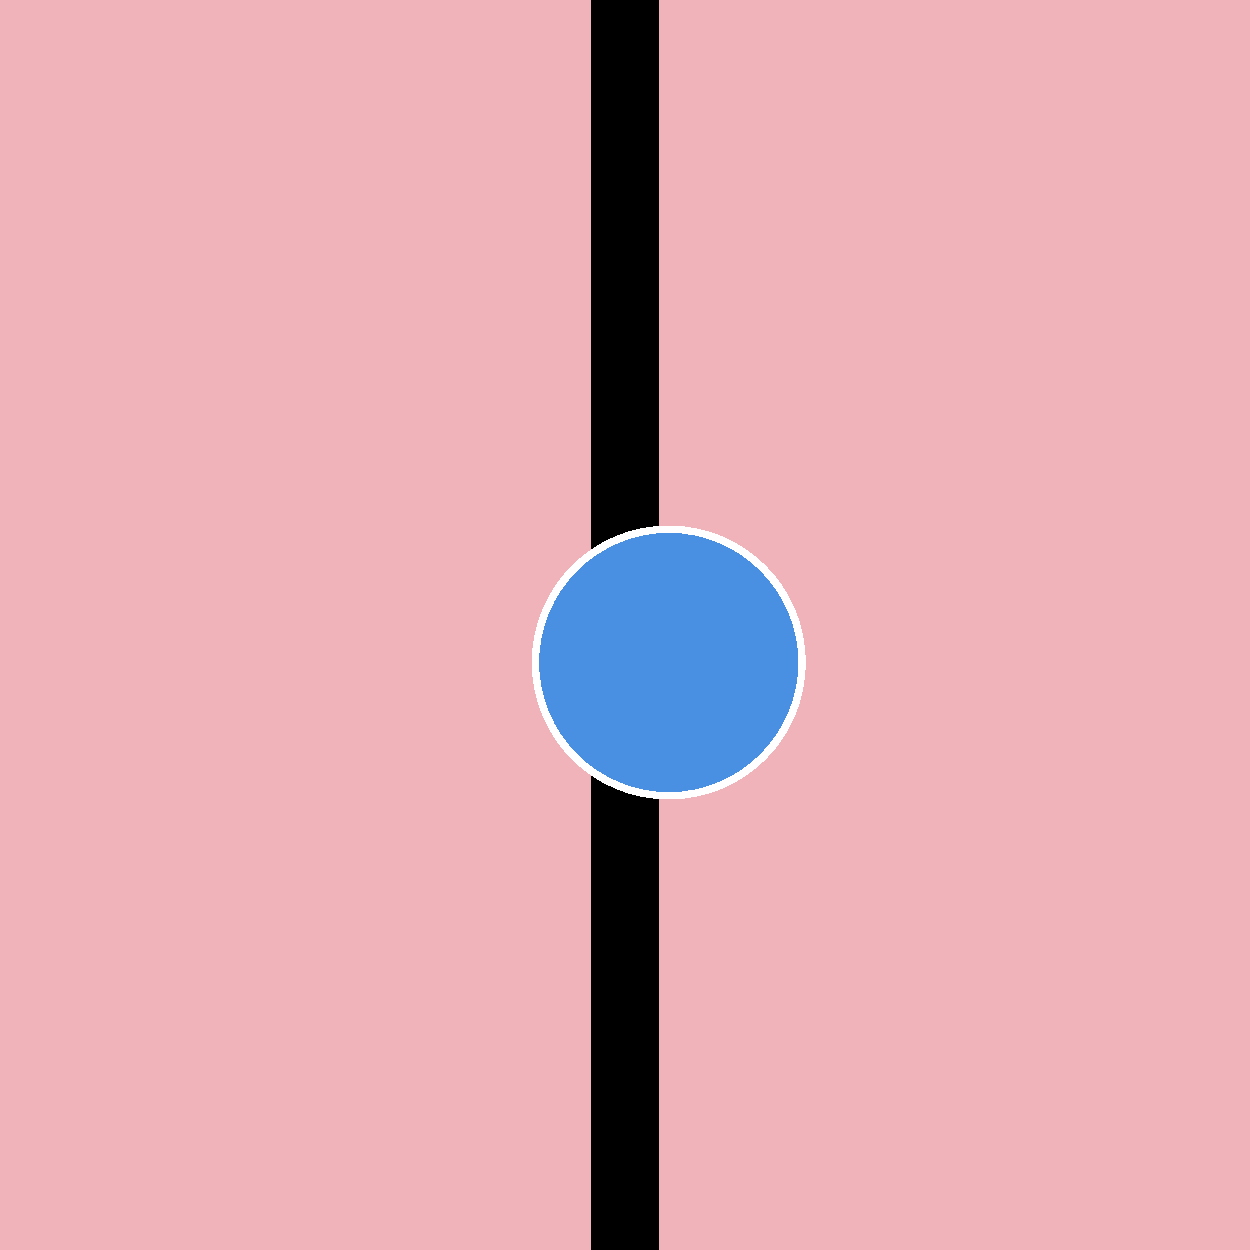
\includegraphics[width=\textwidth]{./resources/worst-case/worst-case-1.pdf}
        \caption{Areas after one split}
        \label{fig:worst-case:one}
    \end{subfigure}
    \hfill
    \begin{subfigure}[t]{0.11\textwidth}
        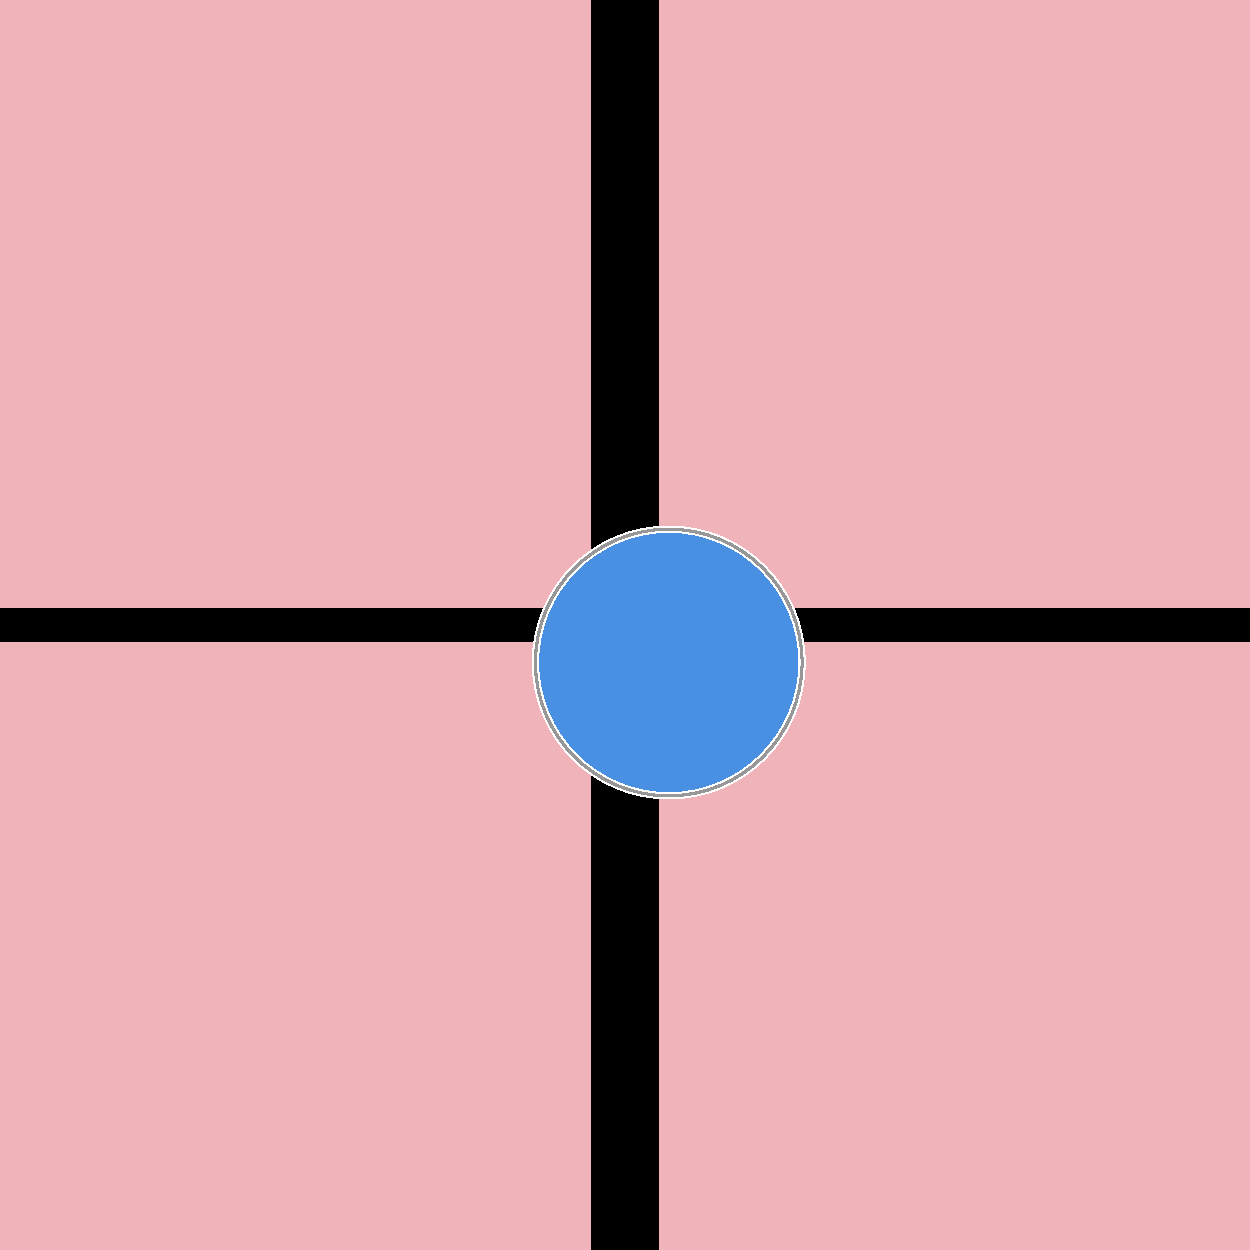
\includegraphics[width=\textwidth]{./resources/worst-case/worst-case-2.pdf}
        \caption{Areas after two splits}
        \label{fig:worst-case:two}
    \end{subfigure}
    \hfill
    \begin{subfigure}[t]{0.11\textwidth}
        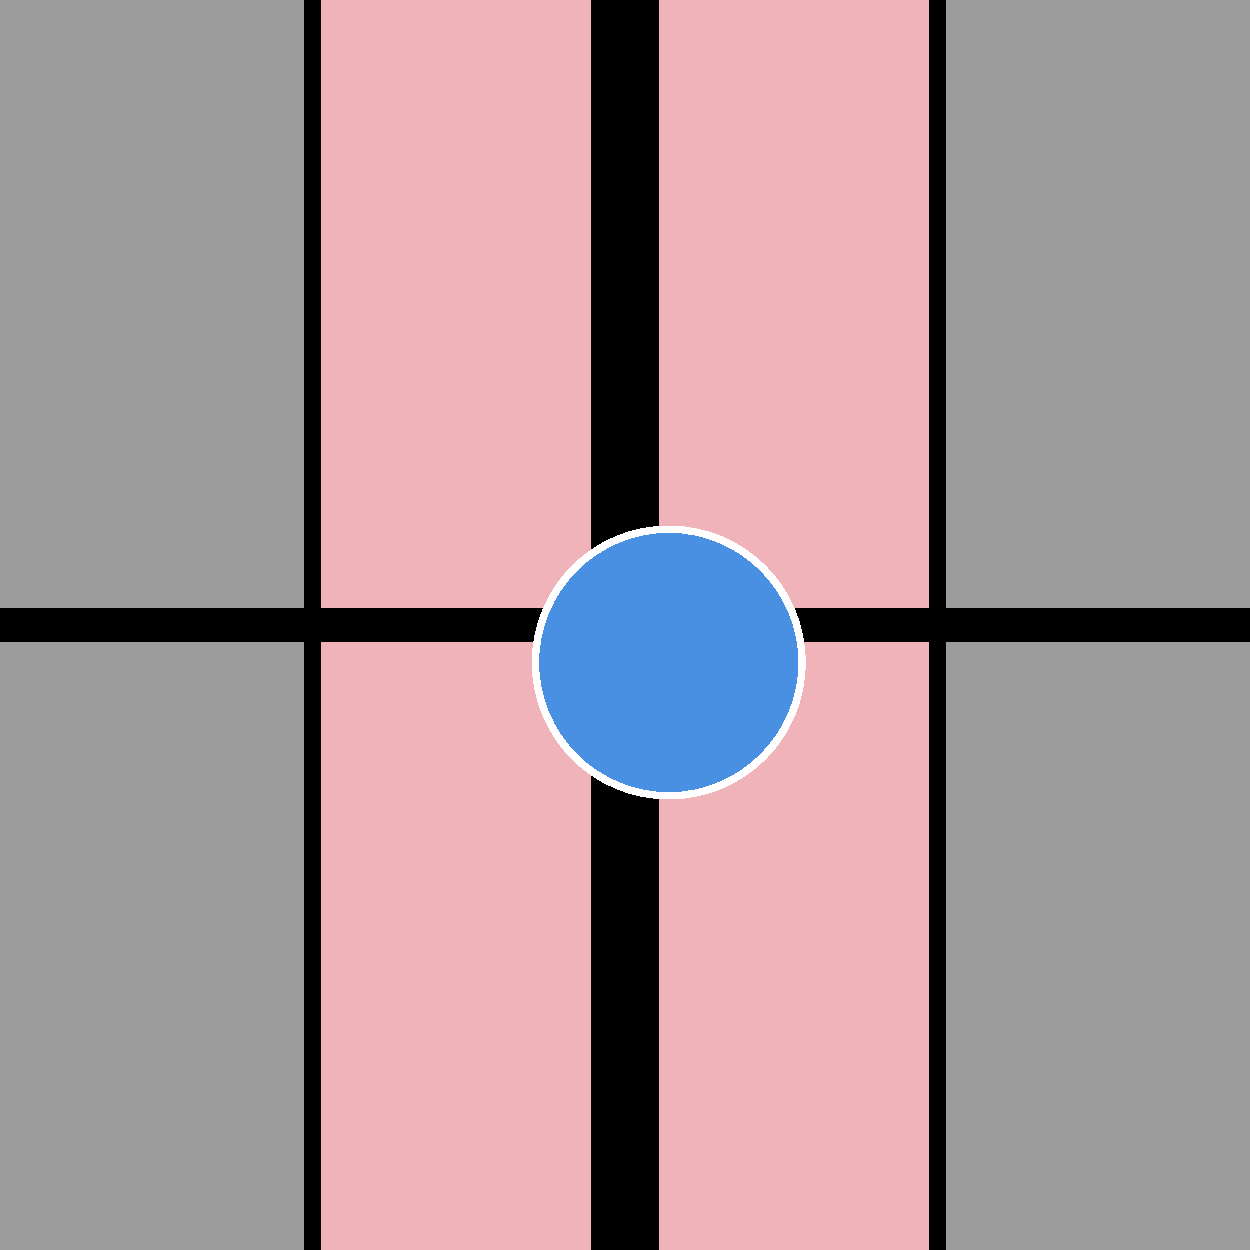
\includegraphics[width=\textwidth]{./resources/worst-case/worst-case-3.pdf}
        \caption{Areas after three splits}
        \label{fig:worst-case:three}
    \end{subfigure}
    \hfill
    \begin{subfigure}[t]{0.11\textwidth}
        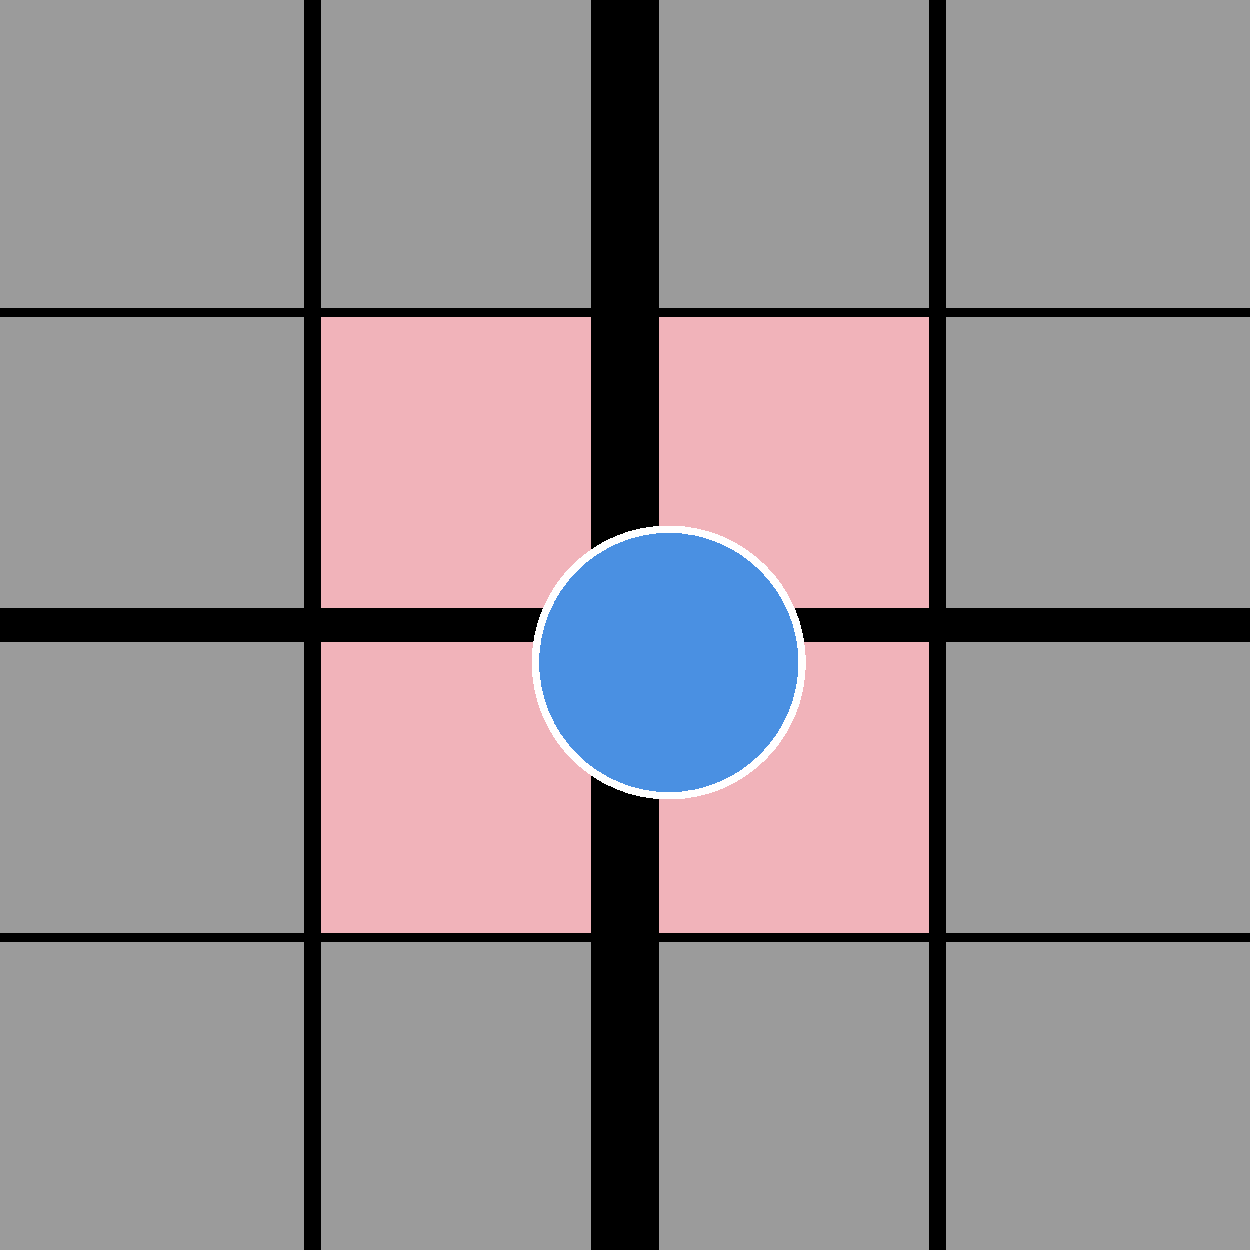
\includegraphics[width=\textwidth]{./resources/worst-case/worst-case-4.pdf}
        \caption{Areas after four splits}
        \label{fig:worst-case:four}
    \end{subfigure}
    \caption{
    	The two-dimensional surface (longitude, latitude) after the first, second, third and fourth split.
    	The blue circle shows a possible area to be claimed by a certificate or the desired query area of a client.
    	The area colored in red is the minimum area that has to be retrieved using the given number of splits.
    }
    \label{fig:worst-case}
\end{figure}

The discretization used by GeoPKI does not directly fit all requirements.
On one hand, claimed volumes will likely never fit exactly one of the voxels.
Moreover, clients likely want to query volumes not aligning with the GeoPKI voxels. 

In both cases this volume $V$ has to be approximated using the GeoPKI voxels.
A trivial approximation the smallest volume encompassing all of $V$.
Unfortunately this results in returning the whole tree if $V$ lies at the intersection of one of the first few division lines.
\Cref{fig:worst-case} depicts this situation with the blue circle corresponding to $V$ and the red area the minimum area that has to be retrieved at the different levels in the tree.
\Cref{fig:worst-case:one} shows the line of the first split.
Given the blue circle intersects both area, the above trivial approximation would result in the whole tree being returned for a comparable small area that is just placed unfortunately.

Thus a better approximation is required.
The main problem with the trivial approximation is the discrepancy of the area queried and the returned area:
If the client queries for a large area, it is fine to return a lot of data.
But in case of a query for a small area, the size of the returned data should be in relation to the queried area.
Given the split lines do not move when going to a deeper level in the tree, it is always necessary to return multiple voxels.
The number of required voxels is monotonically increasing when going deeper down in the tree but the area covered by them monotonically decreases as the voxel approximation for $V$ becomes more accurate.
With decreasing area, the data that has to be returned also monotonically decreases as the subtrees contain at most as much data as any of their super-trees.

\subsubsection{Claimed Volumes to Voxels}

In case of the placement of certificates in the tree, it is infeasible to place certificates claiming a volume $V$ in all leaves covered by $V$ due to the loss in sparsity and the resulting explosion in storage requirements.
As noted before, most places on earth are claimed by at least one country and thus the tree would not be sparse at all.

A plausible heuristic balancing the returned data size with the number of subtrees loss in sparsity is to use a subtree level where the volume of $V$ is greater than or equal to a given fraction $f \in [0,1)$ of the voxel volumes at this level.
For instance $f = \frac{1}{4}$ would result in \Cref{fig:worst-case:three} and $f = \frac{1}{2}$ in \Cref{fig:worst-case:four} (assuming all shown areas cover the full altitude spectrum).
The effectiveness of this heuristic and a good value for $f$ is to be determined using empirical experiments.

\subsubsection{Query to Voxels}

For the transformation of queries to voxels to be queried the case turns out to be easier.
In terms of response size it is always best to retrieve all individual leafs as directly querying a area higher up in the tree will always be a superset of that data.

% First a set of bit strings is defined to \emph{cover} a volume if and only if the union of the results returned when querying each of them contains all certificates intersecting said volume.

%Proof:
%
%Let $V$ be the volume queried by the client and let $S$ be the smallest set of leaf bit strings that covers $V$.
%This set exists as the set of all leaves covers any volume that can be queried.
%The set $S$ is also unique since for each leaf it is possible to individually determine whether it has to be part of $S$. Next, assume there is some distinct set of bit strings $S' \neq S$ covering $V$.
%
%\textbf{Case 1}:
%Assume $S'$ contains only leaf bit strings.
%Since both cover $V$ and $S'$ is the smallest to do so, $S'$ must be a subset of $S$.
%Hence querying $S'$ will return at least as much data as querying $S$ would.
%%Moreover since $S \neq S'$, $S'$ must include at least one leaf whose geometric representation does not intersect $V$ (if it would it would also be part of $S$).
%
%\textbf{Case 2:}
%Assume $S'$ \textbf{not} only contains leaf bit strings.
%Then $S'$ must contain at least one bit string referring to a non-leaf.
%
%\textbf{Case 2a}: Assume all leaf bit strings descendant of all non-leaf nodes are in $S$.
%Then the covered volume is the same and the returned data is exactly the same:
%Querying a larger area rooted at an intermediate node $v$ returns it's full subtree and thus all certificates stored at its descendant leaves.
%Similarly, when directly querying all leaves of an intermediate node $v$ amounts to the same full subtree rooted at $v$ if duplicate intermediate nodes are omitted.
%In both cases the complementary hashes to the root node are required.
%
%\textbf{Case 2b:} Assume \textbf{not} all leaf bit strings descendant of all non-leaf nodes are in $S$.
%Then there is at least one non-leaf node that with a descendant leaf whose bit string is not part of $S$.
%The certificates returned when querying $S$ is thus a subset of the certificates returned when querying $S'$.
%In case the additional voxels covered by $S'$ are all empty, the exact same set of certificates is returned but the proof of absence of the empty nodes are not required when querying $S$.
%In case one of the voxels is non-empty, this is additional data only returned when querying $S'$ but not when querying $S$.
%Moreover these non-intersecting subtrees that at least contain one certificate of $\approx 2$kB size can be replaced by a $32$B hashes for the proof when querying $S$ rather than $S'$.
%
%Since no set $S'$ with a smaller response size can exist, $S$ is optimal.
%
%The question of how to map a point in space and radius to the set of bit strings remains but at least it is now clear what the answer should be.

\subsection{Proofs of Presence and Absence}
\label{sec:data-structure:precense-absence}
Given a query for a volume $V$, the map server should prove that the returned data is in fact in the SMT and that no certificate was omitted.
As described in \Cref{sec:data-structure:query}, the server directly only supports queries for bit strings that have a unique corresponding node $v$ in the SMT.
Let $\mathcal{C}$ with $C \in \mathcal{C}$ be the set of all certificates stored at $v$.
The server has to send the set $\{H(x) \: | \: \forall x \in \mathcal{C} \backslash \{C\}\}$ to the client as it is required to compute the node's hash (see Equations \ref{eq:hash-leaf} and \ref{eq:hash-certs-intermediate-node}).
As described in \Cref{sec:data-structure:query}, if $v$ is an intermediate node, the query result will include the whole subtree rooted at $v$.
Hence a client has all information to compute the hashes of $v$'s children by themselves.
These are required to compute the hash of an intermediate node (see Equation \ref{eq:hash-intermediate-node}).

What is left to complete the proof is the set of complementary hashes along the way to the root and the root hash itself as in a standard SMT.
Since in GeoPKI the intermediate nodes along the way to the root also have associated certificates, the set of their hashes is also required but as specified in \Cref{sec:data-structure:query}, this information is returned to the client anyway and can thus be computed locally.

In a sparse SMT, proving the absence of any certificate in a subtree rooted at $v$ is the same as proving the presence of an empty node.
Thus when a client receives a shorted path up to the root than expected, it already has all information required to proof the node's absence in the tree.

Given the binary SMT has $2^{B}$ leaves (see \Cref{sec:data-structure}), it's depth is $B$.
A proof of presence for a node $v$ at depth $d \in \{0, ..., B-1\}$ (zero is the root itself) then consists of the $d$ complementary node's hash along the path to the root.
The size of these hashes is $256$ bits or $32$ bytes due to the use of SHA-256.
Thus in the worst case a proof for a single leaf consists $\left(B-1\right) \cdot 32$~B $= 66 \cdot 32$~B $= 2'112$~B $\approx 2$~kB and is thus in the same order as an average X.509 certificate.
The size of such a proof is smaller the sparser the tree is and is always smaller if an intermediate node, i.e., not a leaf, is queried.

\subsection{Proof of Consistency}
\label{sec:data-structure:consistency}
As in F-PKI~\cite{chuat_f-pki_2022} using a consistency tree over the root hashes.

\section{Server Implementation}
\label{sec:implementation}

Due to the size of data it seems reasonable to use a data management engine on the server's side, storing the whole data structure in memory is infeasible at the time of writing.

\subsection{Querying for a Sphere Efficiently}
\label{sec:implementation:query-sphere}

\begin{figure}
	\centering
    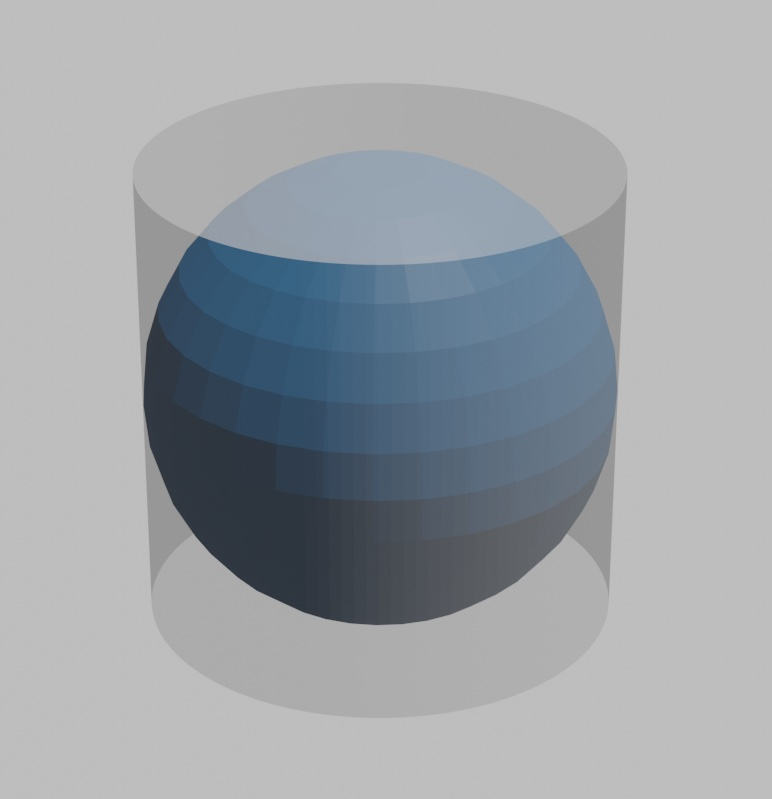
\includegraphics[width=0.25\linewidth]{./resources/query-approximation/cylinder}
    
    \caption{
    	Approximating a sphere using a cylinder.
    }
    \label{fig:sphere-approximation}
\end{figure}

One possibility to query a sphere is to walk the tree and intersect it with the volumes on each level of the tree.
This process is repeated recursively until the reached level is a (sparse) ``leaf''.
When walking the tree like this, all information that has to be returned (including the data for the proof) is obtained in one go.
The database management systems MySQL and PostgreSQL could be extended with a custom index performing the just described operations but they already have built-in support for spatial indexes.

Both have support for two dimensional geodetic coordinates, PostgreSQL additionally supports three dimensional cartesian coordinates but none of them supports two dimensional geodetic coordinates plus a third cartesian altitude dimension.
Transforming points to earth-centered, earth-fixed (ECEF) cartesian coordinates is straight-forward but the same does not apply to volumes since the coordinate system's grid lines are different.
In the geodetic coordinate systems grid lines are curved while in a cartesian coordinate system they are straight lines.
Hence the shape of volumes defined by their vertices is wildly different and would need to be over-approximated when wanting to use the three dimensional spatial index.
While possible, such over-approximations do not seem to be trivial to compute. 

Alternatively it is possible to directly make us of the two-dimensional spatial index with support for geodetic coordinates.
In this approach the altitude is initially completely ignored and the voxel's two dimensional projection to the earth's surface is intersected with a circle with the sphere's radius whose center is the sphere's center also projected to earth's surface.
After querying the spatial index for this, the returned data can be filtered based on the altitude.
Note that this type of query no longer searches for volumes intersecting a sphere but rather over-approximates the sphere as an extruded circle, i.e. a cylinder (see \Cref{fig:sphere-approximation}).
Due to the projection to the earth's surface, the radius of the cylinder has to be adjusted.
When projecting two-dimensional shapes defined by vertices from higher altitudes to the earth's surface (by keeping the longitude and latitude but omitting the altitude), their area shrinks.
Geodetic coordinates simply express the location on the two-dimensional ellipsoid surface where with increasing altitude the corresponding ellipsoid and thus surface area grow.
Analogously when projecting shapes at negative altitudes, their area grows.
This needs to be taken into account when performing the intersection with a circle on earth's surface.
Assuming the original sphere that is queried for is below WGS84's ellipsoid surface and has a radius $r$, the radius used for computing the intersection on earth's surface has to be greater than $r$ since the distance between the sphere's center and all other points on that altitude has increased.
Analogously, the radius can be decreased if the sphere's altitude is above the ellipsoids surface but in this case it is not necessarily required as over-approximating the result is fine when only considering correctness.
Since it is the distances and not areas or volumes that are of interest, the circumferences of ellipses with the different radii should be compared.
Given there is no easy formula for the circumference of an ellipse, the difference is over-approximated by considering spheres instead.
The circumference of an ellipsoid is greater than the circle with a radius corresponding to the length of the ellipse's semi-minor axis ($b$ for WGS84).
Similarly, an ellipsoids circumference is smaller than the circle with a radius corresponding to the length of the ellipse's semi-major axis ($a$ for WGS84).
Thus the fraction by which distances grow from altitude $h$ with $h < 0$ to the earth's surface can be over-approximated as
\begin{align}
\begin{split}
	&\frac{\text{circumference of WGS84 ellipse at }z=0}{\text{circumference of WGS84 ellipse at }z=h}\\
	&\leq \frac{\text{circumference of circle with radius } a}{\text{circumference of circle with radius } (b+h)}\\
	&= \frac{2 a \pi}{2 (b+h) \pi} = \frac{a}{b+h}\\
	&\\
\end{split}
\end{align}

For $h = D$ this results in $\leq 1.005$.

Analogously the fraction by which distances shrink from altitude $h$ with $h > 0$ to the earth's surface can be over-approximated as
\begin{align}
\begin{split}
	&\frac{\text{circumference of WGS84 ellipse at }z=h}{\text{circumference of WGS84 ellipse at }z=0}\\
	&\leq \frac{\text{circumference of circle with radius } (a+h)}{\text{circumference of circle with radius } b}\\
	&= \frac{2 (a+h) \pi}{2 b \pi} = \frac{a+h}{b}\\
	&\\
\end{split}
\end{align}

For $h = H$ this results in $\leq 1.007$.
Given the small numbers and the fact that an over-approximation of the result does not affect correctness, a simple implementation could simply consist of multiplying the radius by $1.005$ to account for possible false negatives.
It is probably advisable to account for this on the client's side to facilitate auditing.
Otherwise a server might claim to not be malicious but return wrong results due to wrong approximations.

\subsection{Database Tables and Schemas}
\label{sec:implementation:schemas}

When using a 2D spatial index as described in \Cref{sec:implementation:query-sphere}, the tables \texttt{nodes} and \texttt{certificates} are used.
The table \texttt{nodes} has the following columns:
\begin{itemize}
	\item \texttt{bit\_string} of type \texttt{bit varying (66)}
	
	Stores the bit strings described in Sections \ref{sec:data-structure:leaf-binary} and \ref{sec:data-structure:intermediate}.
	The table is clustered by the value resulting in geographically close rows being stored somewhat close together on disk.
	\item \texttt{area} of type \texttt{geography}
	
	Stores the 2D projection of the voxel corresponding to the row's \texttt{bit\_string} in the database's internal format.
	There is a 2D spatial index on this column.
	\item \texttt{altitude\_min} of type \texttt{smallint | null}
	
	Stores the minimum altitude corresponding to the row's \texttt{bit\_string}.
	\item \texttt{altitude\_max} of type \texttt{smallint | null}
	
	Stores the maximum altitude corresponding to the row's \texttt{bit\_string}.
	\item \texttt{certificate\_hashes} of type \texttt{bytea[]}
	
	Stores the hashes of the certificates belonging to this node and is by default an empty array.
	The hashes are foreign keys to the \texttt{certificates} table.
	\item \texttt{neighbor\_hash} of type \texttt{bytea | null}
	
	Stores the hash of the node corresponding to the row's neighbor in the SMT (flipping the last bit in the row's bit string) if it is non-empty and otherwise is equal to null.
	This hash might be required for the SMT proof when this row is retrieved.
	\item \texttt{left\_child\_hash} of type \texttt{bytea | null}
	
	Stores the hash of the node corresponding to the row's left child in the SMT (adding a $0$ to the row's bit string) if it is non-empty and otherwise is equal to null.
	This hash might be required for the SMT proof when this row is retrieved.
	\item \texttt{right\_child\_hash} of type \texttt{bytea | null}
	
	Stores the hash of the node corresponding to the row's right child in the SMT (adding a $1$ to the row's bit string) if it is non-empty and otherwise is equal to null.
	This hash might be required for the SMT proof when this row is retrieved.
\end{itemize}

All columns other than \texttt{bit\_string} and \texttt{certificate\_hashes}, are redundant and could be computed based on other information inside the database but are stored explicitly to speed up queries.
To ensure consistency, constraints and triggers are used wherever possible.

The \texttt{certificates} table only consists of two columns, the primary key \texttt{certificate\_hash} of type \texttt{bytea} storing the SHA256 hash of the certificate and the column \texttt{certificate}, also of type \texttt{bytea}, storing the certificate itself.

\section{Optimizations}
\label{sec:optimizations}

First of all it should be noted that the asymmetric design of the bit string with respect to the $z$ dimension allows placing certificates higher in the tree and thus increase sparsity.

Under the assumption most of the world is rather flat with respect to altitude, certificates can often be placed at intermediate nodes covering the full height. % TODO: possibly add citation for "most of the world is flat"
This lowers the tree's height and thus reduces the proof sizes.
For this to work, clients must not expect the certificates to be placed at a unique node in the tree.
The placement does not matter as long as the certificate is stored with \emph{all nodes at one level} whose geometric representation intersect the certificate's claimed volume.
This is because a GeoPKI map server always returns the data along the path to the root together with the whole subtree.
Hence when the certificate is placed in the subtree of the queried volume it will always be included but if it is placed higher in the tree it will only be included if the certificate is stored at one of the parent nodes.

\begin{figure}
    \centering
    \begin{subfigure}[t]{0.11\textwidth}
        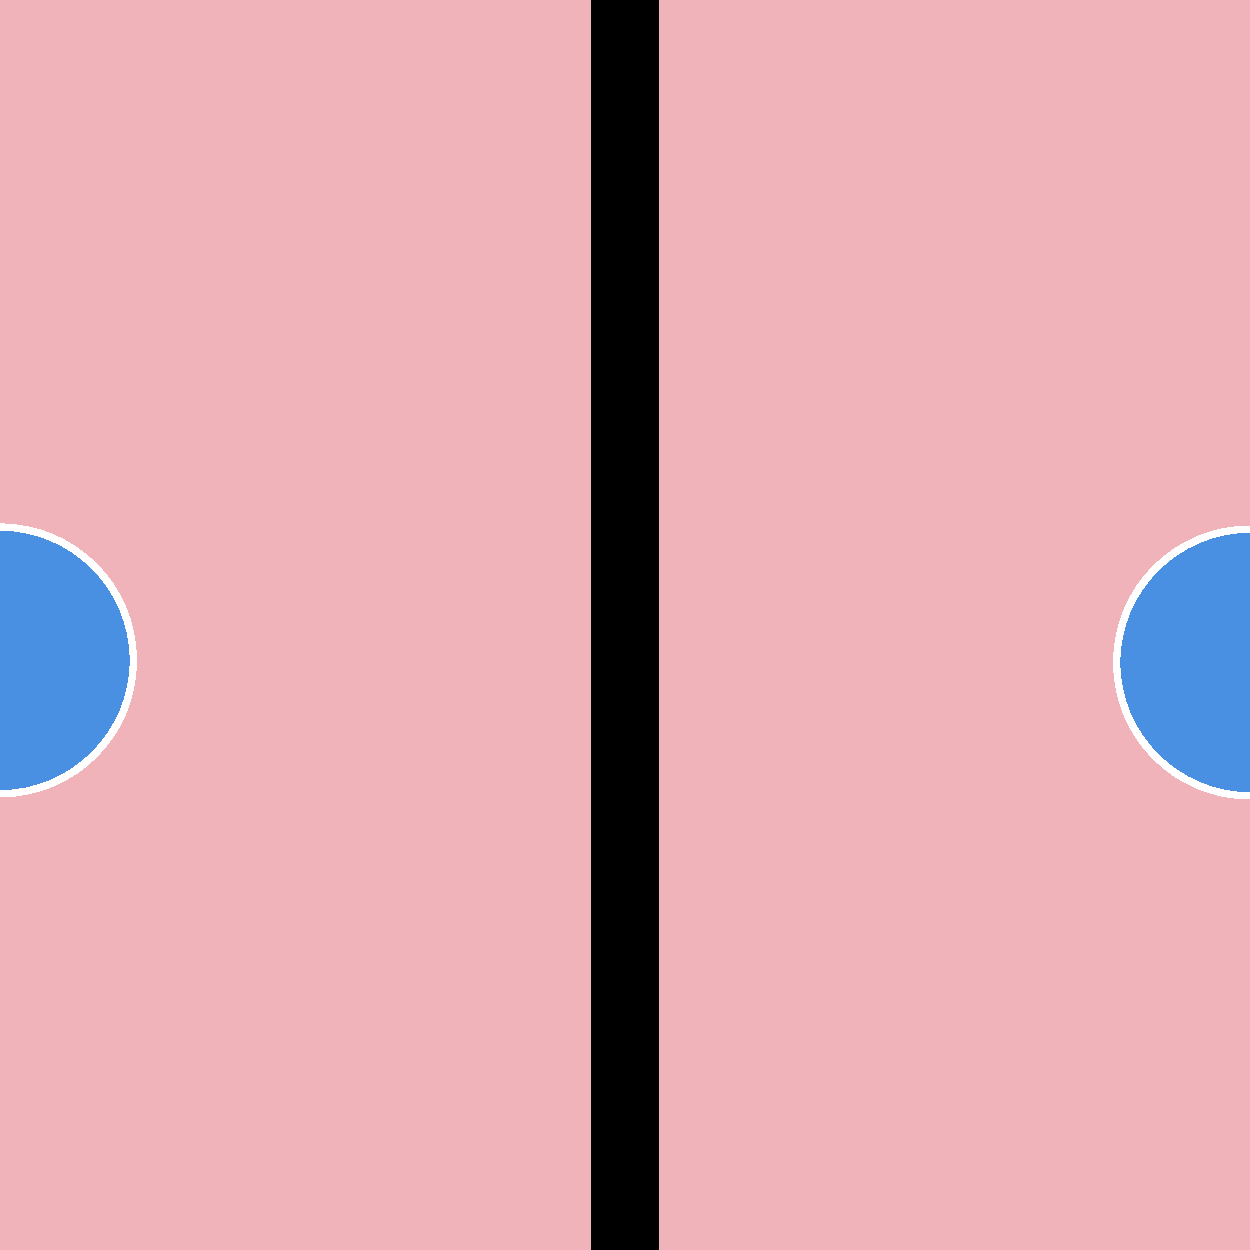
\includegraphics[width=\textwidth]{./resources/worst-case/wrap-around-1.pdf}
        \caption{Areas after one split}
        \label{fig:wrap-around:one}
    \end{subfigure}
    \hfill
    \begin{subfigure}[t]{0.11\textwidth}
        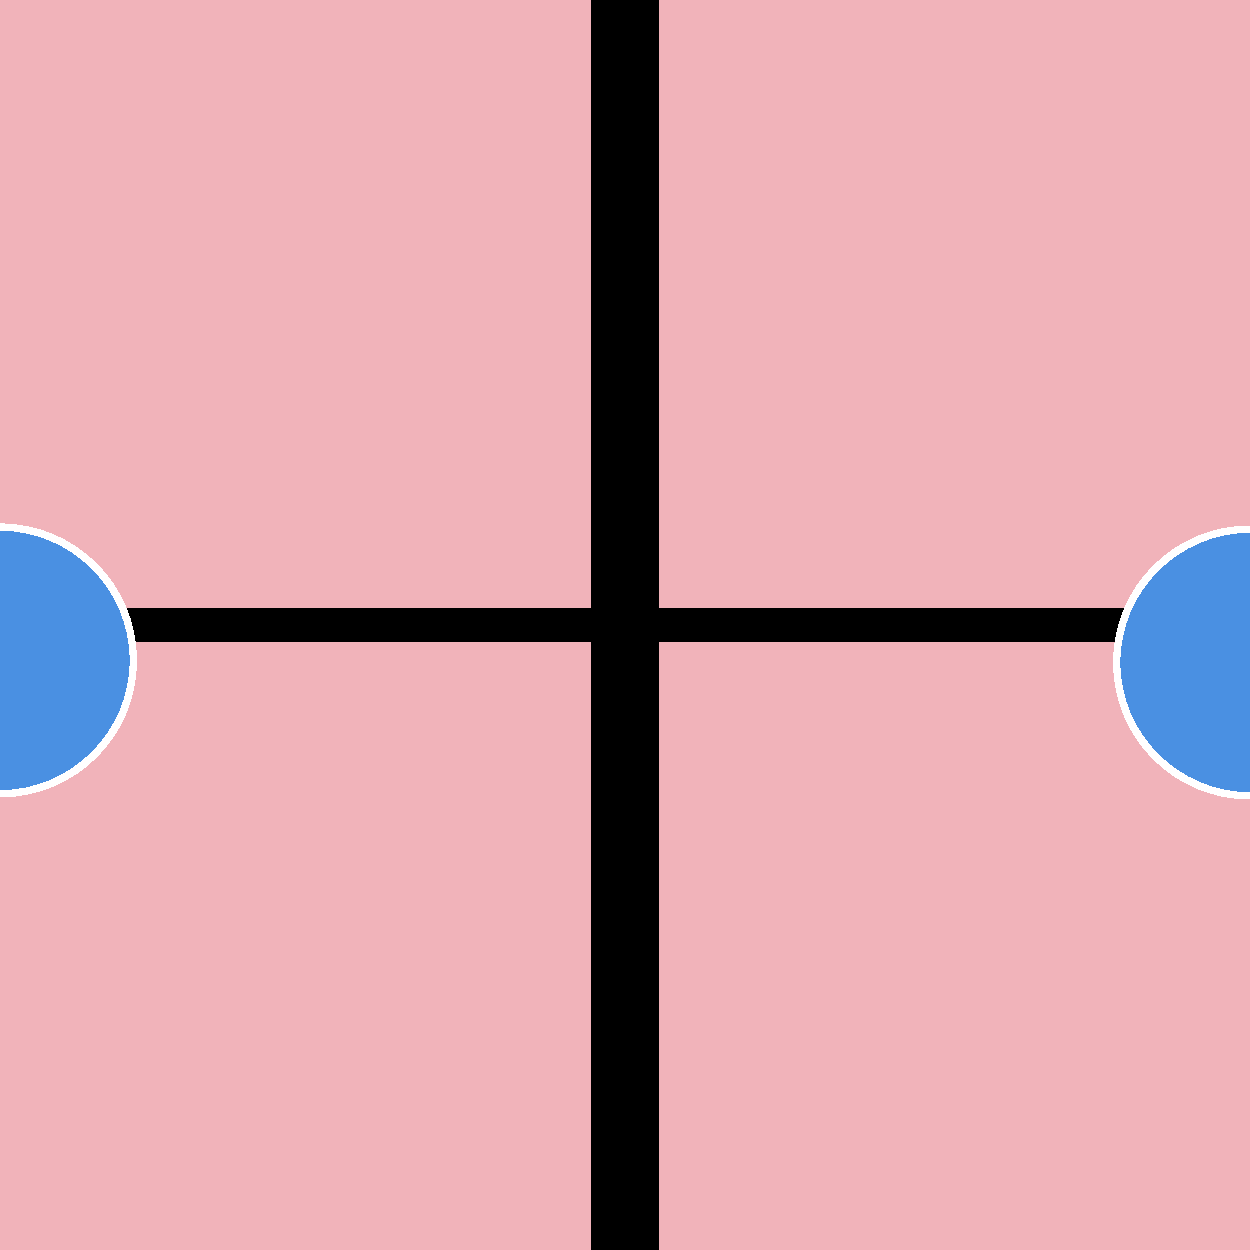
\includegraphics[width=\textwidth]{./resources/worst-case/wrap-around-2.pdf}
        \caption{Areas after two splits}
        \label{fig:wrap-around:two}
    \end{subfigure}
    \hfill
    \begin{subfigure}[t]{0.11\textwidth}
        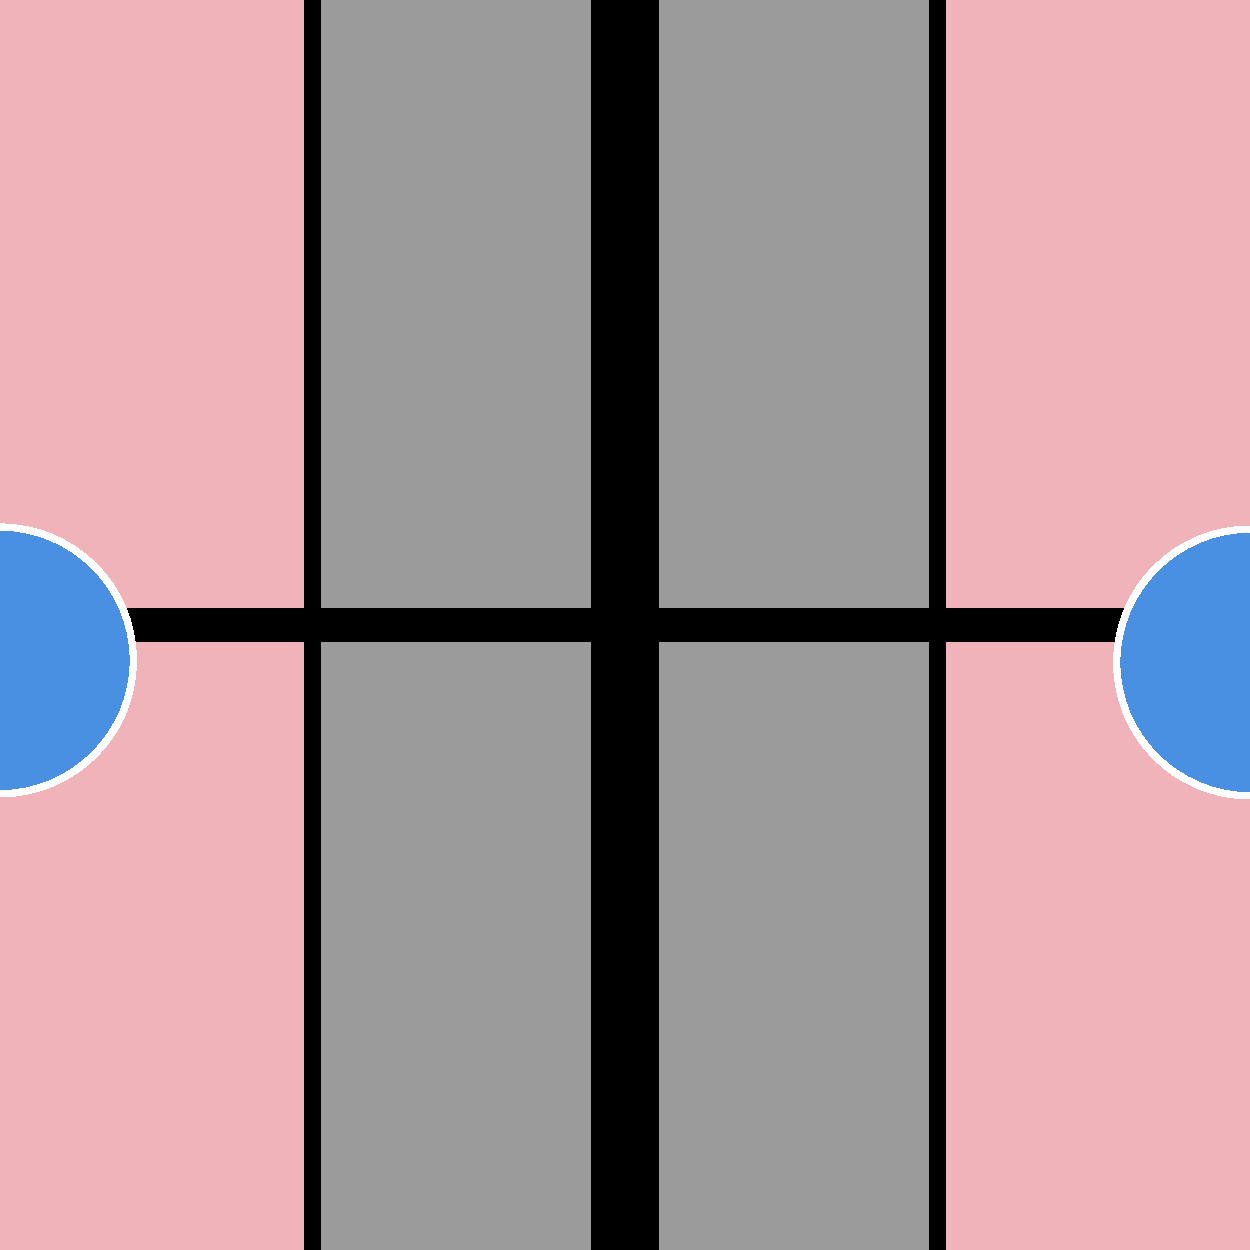
\includegraphics[width=\textwidth]{./resources/worst-case/wrap-around-3.pdf}
        \caption{Areas after three splits}
        \label{fig:wrap-around:three}
    \end{subfigure}
    \hfill
    \begin{subfigure}[t]{0.11\textwidth}
        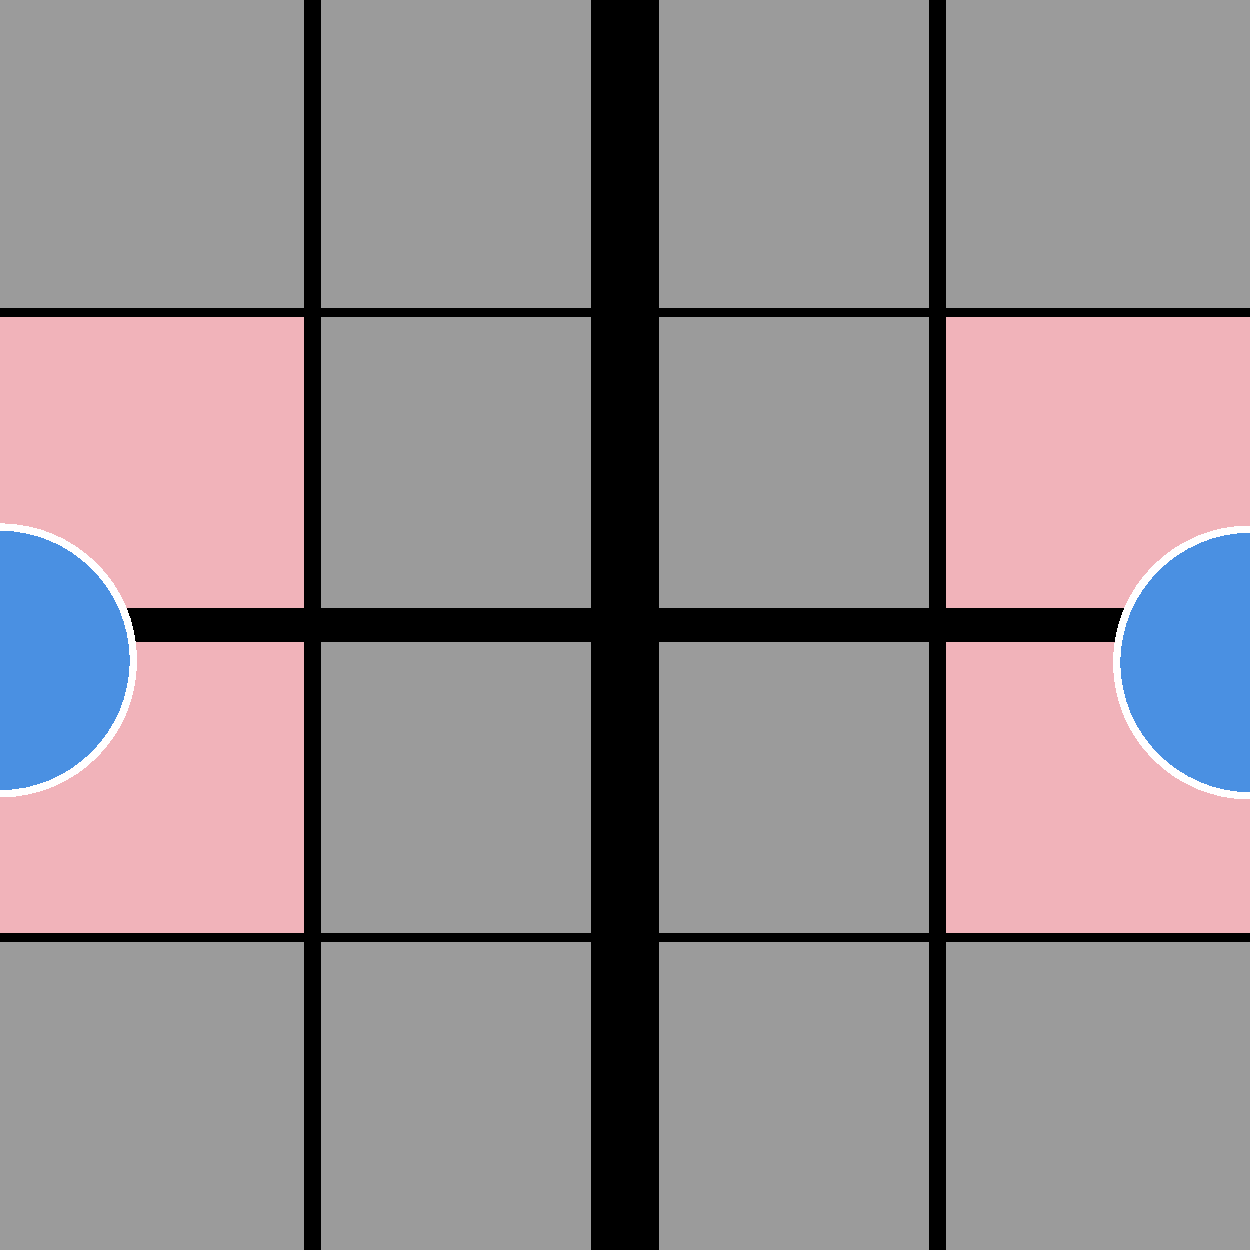
\includegraphics[width=\textwidth]{./resources/worst-case/wrap-around-4.pdf}
        \caption{Areas after four splits}
        \label{fig:wrap-around:four}
    \end{subfigure}
    \caption{
    	The two-dimensional surface (longitude, latitude) after the first, second, third and fourth split.
    	The blue circle shows a possible area to be claimed by a certificate or the desired query area of a client.
    	The area colored in red is the minimum area that has to be retrieved using the given number of splits.
    }
    \label{fig:wrap-around}
\end{figure}

\Cref{sec:data-structure:query} describes how the map server only serves an answer to a single bit string query.
While such an API works, there is room for improvement if correlated queries are answered at the same time.
For instance when the client derives the different bit strings to query a single volume as described in \Cref{sec:data-structure:arbitrary-volumes}, the queries share the path to the root from their lowest common ancestor.
By replying with a single answer for such a set of queries, the data along this shared path has to be returned just once.
Given the use of the Z-order curve (see \Cref{sec:data-structure}) to order the leaves, points spatially close should also be somewhat close in the tree and thus have a common ancestor on lower levels.
Though in the worst case it is still possible that the only common ancestor is the root even if the two areas are spatially close.
This happens when the volume covers both sides of the first split done in the binary tree. This scenario is depicted in \Cref{fig:worst-case:one}.
It seems impossible to avoid such a worst-case scenario entirely when using a tree as described in \Cref{sec:alternative-designs}.

Considering that earth is a sphere and that the coordinates wrap around, the situation becomes even more difficult since a similar situation happens at the points where the coordinate system wraps around.
This scenario is depicted in \Cref{fig:wrap-around}.
This wrap-around can be interpreted as being part of the first split since the problem occurs exactly on the opposite side of the first split when considering the $x$-axis as wrapping around.
To reduce it's impact it would be possible to shift the longitude coordinate system west by $30^{\circ}$.
This way this circle around earth passes through the Atlantic Ocean and Pacific Ocean rather than central Europe.

An additional optimization would be to set $B_y$ to $25$ rather than $26$ bits.
This slightly complicates the notations, definitions and formats but is otherwise straight-forward to implement.

\section{Alternative Designs}
\label{sec:alternative-designs}

An alternative design could use a (hybrid-)quadtree or (hybrid-)octree where most intermediate nodes have four or eight children, respectively.
``Hybrid'' and ``most'' because $B_{x} = B_{y} > B_{z}$ which means the volume cannot be subdivided fully using a quad- or octree.
Hence when using an octree with eight children, the $z$ dimension is already exhausted after $B_{z}$ splits and will from there continue to only have four children (i.e. a quadtree).
When using a quadtree, the first $B_{x,y}$ splits would solely concern the $x$ and $y$ dimensions and after that the children will be binary trees of height $B_{z}$ only splitting the $z$ dimension.
This will decrease the tree's height but increase the proof size due to the larger number of neighboring hashes that have to be provided on each level.
For the hybrid-quadtree, the tree height would be $\log_4(2^{2 \cdot B_{x,y}})= \log_4(4^{B_{x,y}}) = B_{x,y} = 26$ plus the $\log_2(2^{B_z}) = B_z = 15$ for the binary subtrees.
For the hybrid-octree the tree height would be
$\log_8(2^{B_z}) = \log_8(8^{B_z/3}) = B_z/3 = 5$ plus the $\log_4(2^{B - B_z}) = \log_4(2^{2 \cdot B_{x,y}}) = B_{x,y} = 26$ for the quad-subtrees.
The proof size of a leaf would thus increase to $(26 \cdot (4 - 1) + (15 - 1) \cdot (2 - 1)) \cdot 32$~B $= 2'944$~B $\approx$ $3$~kB and $(5 \cdot (8 - 1) + (26 - 1) \cdot (4 - 1)) \cdot 32$~B $= 3'520$~B $\approx$ $3.5$~kB, respectively.
The ones are subtracted from the tree height since the on the last level no complementary hash has to be returned.
The ones subtracted from the number of neighbors is due to the fact that the hash resulting from the leaf itself does not have to be provided as it can be computed by the client.

Unfortunately the worst case scenario remains:
Two spatially adjacent volumes intersecting the lines of the first split only share the root node as a common ancestor.
When using a tree this will always be the case due to nodes having a single parent.
Consider single dimensional discrete consecutive numbers and a binary tree.
Each number (except the start and end) has two numerically neighbors but can only have one neighbor in the tree.
This fact also holds for group of leaves and thus there will always be two numerically close neighbors just sharing the root node as their ancestor.

To maintain consistency with the already introduced binary representation of volumes, one can consider the quad-tree part (i.e. the first $B_{x,y}$ levels) to add two bits to the prefix on each level rather than just one.
The last $B_z$ levels would then each just add a single bit as before.

Since it is not yet clear if and to what extent the usage a more complex tree structure could be beneficial and hence the more simple binary tree is preferred for the moment.

\section{Caveats}
\label{sec:caveats}

Since longitude ($x$) and latitude ($y$) coordinates that are split in half numerically represent polar coordinates on a sphere, numerically equidistant points, areas or volumes are not equidistant on earth.
Near the poles the longitudinal circumference is smaller but represented using the same numerically range resulting in higher precision.
Hence the discretization range was chosen based on the semi-major axis at the equator where the achieved precision is smallest.

\section{Certificate Format}
\label{sec:certificate-format}

The claimed volume has to be specified in the X.509 certificate.
The used format should be flexible enough to support a variety of use cases such as a set of disjoint volumes, rectangular but also circular volumes.
Open Street Maps uses polygons and RFC 7946 specifies the ``geospatial data interchange format'' GeoJSON \cite{butler_geojson_2016} that also makes use of polygons.
One option would be to define additional types allowing for three dimensional polygons, another to use the ``properties'' field defined in RFC 7946.
When going with the latter approach, each certificate could define a \texttt{GeometryCollection} of \texttt{Polygon}s or \texttt{MultiPolygon}s, each with an \texttt{altitude\_from} and \texttt{altitude\_to} property indicating the inclusive minimum and maximum altitude, respectively.
Note that this representation only allows for extruded two dimensional polygons as primitives but their composition allows more complex shapes.
Since the GeoJSON uses a text-encoding, serializing the data using e.g. protocol buffers as done by Mapbox \cite{mapbox_geobuf_2023} will result in a smaller encoding and fast read and write operations.

\bibliographystyle{IEEEtran}
\bibliography{GeoPKI.bib}
\end{document}
